% Options for packages loaded elsewhere
\PassOptionsToPackage{unicode}{hyperref}
\PassOptionsToPackage{hyphens}{url}
%
\documentclass[
]{book}
\usepackage{amsmath,amssymb}
\usepackage{iftex}
\ifPDFTeX
  \usepackage[T1]{fontenc}
  \usepackage[utf8]{inputenc}
  \usepackage{textcomp} % provide euro and other symbols
\else % if luatex or xetex
  \usepackage{unicode-math} % this also loads fontspec
  \defaultfontfeatures{Scale=MatchLowercase}
  \defaultfontfeatures[\rmfamily]{Ligatures=TeX,Scale=1}
\fi
\usepackage{lmodern}
\ifPDFTeX\else
  % xetex/luatex font selection
\fi
% Use upquote if available, for straight quotes in verbatim environments
\IfFileExists{upquote.sty}{\usepackage{upquote}}{}
\IfFileExists{microtype.sty}{% use microtype if available
  \usepackage[]{microtype}
  \UseMicrotypeSet[protrusion]{basicmath} % disable protrusion for tt fonts
}{}
\makeatletter
\@ifundefined{KOMAClassName}{% if non-KOMA class
  \IfFileExists{parskip.sty}{%
    \usepackage{parskip}
  }{% else
    \setlength{\parindent}{0pt}
    \setlength{\parskip}{6pt plus 2pt minus 1pt}}
}{% if KOMA class
  \KOMAoptions{parskip=half}}
\makeatother
\usepackage{xcolor}
\usepackage{color}
\usepackage{fancyvrb}
\newcommand{\VerbBar}{|}
\newcommand{\VERB}{\Verb[commandchars=\\\{\}]}
\DefineVerbatimEnvironment{Highlighting}{Verbatim}{commandchars=\\\{\}}
% Add ',fontsize=\small' for more characters per line
\usepackage{framed}
\definecolor{shadecolor}{RGB}{248,248,248}
\newenvironment{Shaded}{\begin{snugshade}}{\end{snugshade}}
\newcommand{\AlertTok}[1]{\textcolor[rgb]{0.94,0.16,0.16}{#1}}
\newcommand{\AnnotationTok}[1]{\textcolor[rgb]{0.56,0.35,0.01}{\textbf{\textit{#1}}}}
\newcommand{\AttributeTok}[1]{\textcolor[rgb]{0.13,0.29,0.53}{#1}}
\newcommand{\BaseNTok}[1]{\textcolor[rgb]{0.00,0.00,0.81}{#1}}
\newcommand{\BuiltInTok}[1]{#1}
\newcommand{\CharTok}[1]{\textcolor[rgb]{0.31,0.60,0.02}{#1}}
\newcommand{\CommentTok}[1]{\textcolor[rgb]{0.56,0.35,0.01}{\textit{#1}}}
\newcommand{\CommentVarTok}[1]{\textcolor[rgb]{0.56,0.35,0.01}{\textbf{\textit{#1}}}}
\newcommand{\ConstantTok}[1]{\textcolor[rgb]{0.56,0.35,0.01}{#1}}
\newcommand{\ControlFlowTok}[1]{\textcolor[rgb]{0.13,0.29,0.53}{\textbf{#1}}}
\newcommand{\DataTypeTok}[1]{\textcolor[rgb]{0.13,0.29,0.53}{#1}}
\newcommand{\DecValTok}[1]{\textcolor[rgb]{0.00,0.00,0.81}{#1}}
\newcommand{\DocumentationTok}[1]{\textcolor[rgb]{0.56,0.35,0.01}{\textbf{\textit{#1}}}}
\newcommand{\ErrorTok}[1]{\textcolor[rgb]{0.64,0.00,0.00}{\textbf{#1}}}
\newcommand{\ExtensionTok}[1]{#1}
\newcommand{\FloatTok}[1]{\textcolor[rgb]{0.00,0.00,0.81}{#1}}
\newcommand{\FunctionTok}[1]{\textcolor[rgb]{0.13,0.29,0.53}{\textbf{#1}}}
\newcommand{\ImportTok}[1]{#1}
\newcommand{\InformationTok}[1]{\textcolor[rgb]{0.56,0.35,0.01}{\textbf{\textit{#1}}}}
\newcommand{\KeywordTok}[1]{\textcolor[rgb]{0.13,0.29,0.53}{\textbf{#1}}}
\newcommand{\NormalTok}[1]{#1}
\newcommand{\OperatorTok}[1]{\textcolor[rgb]{0.81,0.36,0.00}{\textbf{#1}}}
\newcommand{\OtherTok}[1]{\textcolor[rgb]{0.56,0.35,0.01}{#1}}
\newcommand{\PreprocessorTok}[1]{\textcolor[rgb]{0.56,0.35,0.01}{\textit{#1}}}
\newcommand{\RegionMarkerTok}[1]{#1}
\newcommand{\SpecialCharTok}[1]{\textcolor[rgb]{0.81,0.36,0.00}{\textbf{#1}}}
\newcommand{\SpecialStringTok}[1]{\textcolor[rgb]{0.31,0.60,0.02}{#1}}
\newcommand{\StringTok}[1]{\textcolor[rgb]{0.31,0.60,0.02}{#1}}
\newcommand{\VariableTok}[1]{\textcolor[rgb]{0.00,0.00,0.00}{#1}}
\newcommand{\VerbatimStringTok}[1]{\textcolor[rgb]{0.31,0.60,0.02}{#1}}
\newcommand{\WarningTok}[1]{\textcolor[rgb]{0.56,0.35,0.01}{\textbf{\textit{#1}}}}
\usepackage{longtable,booktabs,array}
\usepackage{calc} % for calculating minipage widths
% Correct order of tables after \paragraph or \subparagraph
\usepackage{etoolbox}
\makeatletter
\patchcmd\longtable{\par}{\if@noskipsec\mbox{}\fi\par}{}{}
\makeatother
% Allow footnotes in longtable head/foot
\IfFileExists{footnotehyper.sty}{\usepackage{footnotehyper}}{\usepackage{footnote}}
\makesavenoteenv{longtable}
\usepackage{graphicx}
\makeatletter
\def\maxwidth{\ifdim\Gin@nat@width>\linewidth\linewidth\else\Gin@nat@width\fi}
\def\maxheight{\ifdim\Gin@nat@height>\textheight\textheight\else\Gin@nat@height\fi}
\makeatother
% Scale images if necessary, so that they will not overflow the page
% margins by default, and it is still possible to overwrite the defaults
% using explicit options in \includegraphics[width, height, ...]{}
\setkeys{Gin}{width=\maxwidth,height=\maxheight,keepaspectratio}
% Set default figure placement to htbp
\makeatletter
\def\fps@figure{htbp}
\makeatother
\setlength{\emergencystretch}{3em} % prevent overfull lines
\providecommand{\tightlist}{%
  \setlength{\itemsep}{0pt}\setlength{\parskip}{0pt}}
\setcounter{secnumdepth}{5}
\usepackage{booktabs}
\usepackage{amsthm}
\makeatletter
\def\thm@space@setup{%
  \thm@preskip=8pt plus 2pt minus 4pt
  \thm@postskip=\thm@preskip
}
\makeatother
\ifLuaTeX
  \usepackage{selnolig}  % disable illegal ligatures
\fi
\usepackage[]{natbib}
\bibliographystyle{apalike}
\IfFileExists{bookmark.sty}{\usepackage{bookmark}}{\usepackage{hyperref}}
\IfFileExists{xurl.sty}{\usepackage{xurl}}{} % add URL line breaks if available
\urlstyle{same}
\hypersetup{
  pdftitle={Introduction to R},
  pdfauthor={Claudia A Engel},
  hidelinks,
  pdfcreator={LaTeX via pandoc}}

\title{Introduction to R}
\author{Claudia A Engel}
\date{Last updated: October 14, 2023}

\begin{document}
\maketitle

{
\setcounter{tocdepth}{1}
\tableofcontents
}
\hypertarget{prerequisites}{%
\chapter*{Prerequisites}\label{prerequisites}}
\addcontentsline{toc}{chapter}{Prerequisites}

\begin{itemize}
\tightlist
\item
  Geared specifically towards users who are \textbf{new} to R.\\
\item
  Have \href{https://cran.r-project.org/}{R} and \href{https://posit.co/download/rstudio-desktop/}{RStudio} installed (see setup instructions below).
\end{itemize}

\hypertarget{setup-instructions}{%
\section*{Setup Instructions}\label{setup-instructions}}
\addcontentsline{toc}{section}{Setup Instructions}

\href{https://cran.r-project.org/}{\textbf{R}} and \href{https://posit.co/download/rstudio-desktop/}{\textbf{RStudio}} are separate downloads and installations. R is the
underlying statistical computing environment. It can be used on its own, but using R alone is no fun. RStudio is a graphical integrated development environment (IDE) that makes using R much easier and more interactive. You need to install R before you launch RStudio.

Be aware that the most recent version of RStudio requires R version 3.3.0 or later.

\hypertarget{macos}{%
\subsection*{macOS}\label{macos}}
\addcontentsline{toc}{subsection}{macOS}

\hypertarget{if-you-already-have-r-and-rstudio-installed}{%
\subsubsection*{If you already have R and RStudio installed}\label{if-you-already-have-r-and-rstudio-installed}}
\addcontentsline{toc}{subsubsection}{If you already have R and RStudio installed}

\begin{itemize}
\tightlist
\item
  Open RStudio, and click on ``Help'' \textgreater{} ``Check for updates''. If a new version is
  available, quit RStudio, and download the latest version for RStudio.
\item
  To check the version of R you are using, start RStudio and the first thing
  that appears on the terminal indicates the version of R you are running. Alternatively, you can type \texttt{sessionInfo()}, which will also display which version of R you are running. Go on
  the \href{https://cran.r-project.org/bin/macosx/}{CRAN website} and check
  whether a more recent version is available. If so, please download and install
  it.
\end{itemize}

\hypertarget{if-you-dont-have-r-and-rstudio-installed}{%
\subsubsection*{If you don't have R and RStudio installed}\label{if-you-dont-have-r-and-rstudio-installed}}
\addcontentsline{toc}{subsubsection}{If you don't have R and RStudio installed}

\begin{itemize}
\tightlist
\item
  Download R from
  the \href{http://cran.r-project.org/bin/macosx}{CRAN website}.
\item
  Select the \texttt{.pkg} file for the latest R version. Make sure you choose the appropriate version for your hardware (Apple silicon or Intel)
\item
  Double click on the downloaded file to install R
\item
  Go to the \href{https://posit.co/download/rstudio-desktop/}{RStudio download page}
\item
  Follow the link to download the latest version under ``Install Rstudio''
\item
  Double click the file to install RStudio
\item
  Once it's installed, open RStudio to make sure it works and you don't get any
  error messages.
\end{itemize}

\hypertarget{windows}{%
\subsection*{Windows}\label{windows}}
\addcontentsline{toc}{subsection}{Windows}

\hypertarget{if-you-already-have-r-and-rstudio-installed-1}{%
\subsubsection*{If you already have R and RStudio installed}\label{if-you-already-have-r-and-rstudio-installed-1}}
\addcontentsline{toc}{subsubsection}{If you already have R and RStudio installed}

\begin{itemize}
\tightlist
\item
  Open RStudio, and click on ``Help'' \textgreater{} ``Check for updates''. If a new version is
  available, quit RStudio, and download the latest version for RStudio.
\item
  To check which version of R you are using, start RStudio and the first thing
  that appears in the console indicates the version of R you are
  running. Alternatively, you can type \texttt{sessionInfo()}, which will also display
  which version of R you are running. Go on
  the \href{https://cran.r-project.org/bin/windows/base/}{CRAN website} and check
  whether a more recent version is available. If so, please download and install
  it. You can \href{https://cran.r-project.org/bin/windows/base/rw-FAQ.html\#How-do-I-UNinstall-R_003f}{check here} for
  more information on how to remove old versions from your system if you wish to do so.
\end{itemize}

\hypertarget{if-you-dont-have-r-and-rstudio-installed-1}{%
\subsubsection*{If you don't have R and RStudio installed}\label{if-you-dont-have-r-and-rstudio-installed-1}}
\addcontentsline{toc}{subsubsection}{If you don't have R and RStudio installed}

\begin{itemize}
\tightlist
\item
  Download R from
  the \href{http://cran.r-project.org/bin/windows/base/release.htm}{CRAN website}.
\item
  Run the \texttt{.exe} file that was just downloaded
\item
  Go to the \href{https://posit.co/download/rstudio-desktop/}{RStudio download page}
\item
  Follow the link to download the latest version under ``Install Rstudio''
\item
  Double click the file to install it
\item
  Once it's installed, open RStudio to make sure it works and you don't get any
  error messages.
\end{itemize}

\hypertarget{linux}{%
\subsection*{Linux}\label{linux}}
\addcontentsline{toc}{subsection}{Linux}

\begin{itemize}
\tightlist
\item
  Follow the instructions for your distribution
  from \href{https://cloud.r-project.org/bin/linux}{CRAN}, they provide information
  to get the most recent version of R for common distributions. For most
  distributions, you could use your package manager (e.g., for Debian/Ubuntu run
  \texttt{sudo\ apt-get\ install\ r-base}, and for Fedora \texttt{sudo\ yum\ install\ R}), but we
  don't recommend this approach as the versions provided by this are
  usually out of date. In any case, make sure you have at least R 4.0.0.
\item
  Go to the \href{https://posit.co/download/rstudio-desktop/}{RStudio download page}
\item
  Follow the link to download the latest version under ``Install Rstudio''
\item
  Once it's installed, open RStudio to make sure it works and you don't get any
  error messages.
\end{itemize}

\hypertarget{acknowledgements}{%
\section*{Acknowledgements}\label{acknowledgements}}
\addcontentsline{toc}{section}{Acknowledgements}

Part of the materials for this tutorial are adapted from \url{http://datacarpentry.org} and \url{http://softwarecarpentry.org}.

\hypertarget{backgroud}{%
\chapter{R and Rstudio}\label{backgroud}}

\begin{quote}
Learning Objectives

\begin{itemize}
\tightlist
\item
  Be familiar with reasons to use R.
\item
  Understand how R relates to RStudio.
\item
  Be able to navigate the RStudio interface including the Script, Console, Environment, Help, Files, and Plots windows.
\item
  Create an R Project in RStudio.
\item
  Set a ``working'' directory.
\item
  Send commands from the Script window to the Console in RStudio.
\item
  Install additional packages with RStudio and using R commands.
\end{itemize}
\end{quote}

\begin{center}\rule{0.5\linewidth}{0.5pt}\end{center}

\hypertarget{what-is-r-what-is-rstudio}{%
\section{What is R? What is RStudio?}\label{what-is-r-what-is-rstudio}}

The term ``R'' is used to refer to both the programming language to write scripts and the software (``environment'') that interprets the scripts written in R. It is an alternative to statistical packages like SAS, SPSS, or Stata, which lets you perform a wide variety of data analysis, statistics, and visualization.

RStudio is currently a very popular way to not only write your R scripts but
also to interact with the R software. To function correctly, RStudio needs R and therefore both need to be installed on your computer.

\hypertarget{why-learn-r}{%
\section{Why learn R?}\label{why-learn-r}}

\hypertarget{r-does-not-involve-lots-of-pointing-and-clicking-and-thats-a-good-thing}{%
\subsection{R does not involve lots of pointing and clicking, and that's a good thing}\label{r-does-not-involve-lots-of-pointing-and-clicking-and-thats-a-good-thing}}

The learning curve might be steeper than with other software, but with R, the
results of your analysis does not rely on remembering a succession of pointing
and clicking, but instead on a series of written commands, and that's a good
thing! So, if you want to redo your analysis because you collected more data,
you don't have to remember which button you clicked in which order to obtain
your results, you just have to run your script again.

Working with scripts makes the steps you used in your analysis clear, and the
code you write can be inspected by someone else who can give you feedback and
spot mistakes.

Working with scripts forces you to have a deeper understanding of what you are
doing, and facilitates your learning and comprehension of the methods you use.

\hypertarget{r-code-is-great-for-reproducibility}{%
\subsection{R code is great for reproducibility}\label{r-code-is-great-for-reproducibility}}

Reproducibility is when someone else (including your future self) can obtain the
same results from the same dataset when using the same analysis.

R integrates with other tools to generate manuscripts from your code. If you
collect more data, or fix a mistake in your dataset, the figures and the
statistical tests in your manuscript are updated automatically.

An increasing number of journals and funding agencies expect analyses to be
reproducible, so knowing R will give you an edge with these requirements.

\hypertarget{r-is-multidisciplinary-extensible-and-popular}{%
\subsection{R is multidisciplinary, extensible, and popular}\label{r-is-multidisciplinary-extensible-and-popular}}

With \href{https://cran.r-project.org/web/packages}{close to 20,000 packages on CRAN} (The Comprehensive R Archive Network) that can be installed to extend its capabilities, R
provides a framework that allows you to combine statistical approaches from many
scientific disciplines to best suit the analytical framework you need to analyze your
data. For instance, R has packages for image analysis, mapping, time series, text mining, and a lot more.

\hypertarget{r-works-on-data-of-all-shapes-and-sizes}{%
\subsection{R works on data of all shapes and sizes}\label{r-works-on-data-of-all-shapes-and-sizes}}

The skills you learn with R scale easily with the size of your dataset. Whether
your dataset has hundreds or millions of lines, it won't make much difference to
you.

R is designed for data analysis. It comes with special data structures and data
types that make handling of missing data and statistical factors convenient.

R can connect to spreadsheets, databases, and many other data formats, on your
computer or on the web.

\hypertarget{r-produces-high-quality-graphics}{%
\subsection{R produces high-quality graphics}\label{r-produces-high-quality-graphics}}

The plotting functionalities in R are endless, and allow you to adjust any
aspect of your graph to convey most effectively the message from your data.

\hypertarget{r-has-a-large-user-community}{%
\subsection{R has a large user community}\label{r-has-a-large-user-community}}

Thousands of people use R daily. Many of them are willing to help you through
mailing lists and websites such as \href{https://stackoverflow.com/questions/tagged/r}{Stack Overflow}.

\hypertarget{not-only-is-r-free-but-it-is-also-open-source-and-cross-platform}{%
\subsection{Not only is R free, but it is also open-source and cross-platform}\label{not-only-is-r-free-but-it-is-also-open-source-and-cross-platform}}

Anyone can inspect the source code to see how R works. Because of this
transparency, there is less chance for mistakes, and if you (or someone else)
find some, you can report and fix bugs.

\hypertarget{knowing-your-way-around-rstudio}{%
\section{Knowing your way around RStudio}\label{knowing-your-way-around-rstudio}}

Let's start by learning about \href{https://www.rstudio.com/}{RStudio}, which is an
Integrated Development Environment (IDE) for working with R.

The RStudio IDE open-source product is free under the
\href{https://www.gnu.org/licenses/agpl-3.0.en.html}{Affero General Public License (AGPL) v3}.
The RStudio IDE is also available with a commercial license and priority email
support from RStudio, Inc.

We will use RStudio IDE to write code, navigate the files on our computer,
inspect the variables we are going to create, and visualize the plots we will
generate. RStudio can also be used for other things (e.g., version control,
developing packages, writing Shiny apps) that we will not cover during the
workshop.

\begin{figure}
\includegraphics[width=1\linewidth]{img/rstudio-screenshot} \caption{The RStudio Interface}\label{fig:RStudio-GUI}
\end{figure}

RStudio is divided into 4 ``Panes'':

\begin{itemize}
\tightlist
\item
  the \textbf{Source} for your scripts and documents
  (top-left, in the default layout),
\item
  the R \textbf{Console} (bottom-left),
\item
  your \textbf{Environment/History} (top-right), and
\item
  your \textbf{Files/Plots/Packages/Help/Viewer} (bottom-right).
\end{itemize}

The placement of these
panes and their content can be customized (see main Menu, Tools -\textgreater{} Global Options -\textgreater{}
Pane Layout). One of the advantages of using RStudio is that all the information
you need to write code is available in a single window.

\hypertarget{how-to-start-an-r-project}{%
\section{How to start an R project}\label{how-to-start-an-r-project}}

It is good practice to keep a set of related data, analyses, and text
self-contained in a single folder. When working with R and RStudio you typically want that single top folder to be the folder you are working in. In order to tell R this, you will want to set that folder as your \textbf{working directory}. Whenever you refer to other scripts or data or directories contained within the working directory you can then use \emph{relative paths} to files that indicate
where inside the project a file is located. (That is opposed to absolute paths, which
point to where a file is on a specific computer). Having everything contained in a single directory makes it
a lot easier to move your project around on your computer and share it with
others without worrying about whether or not the underlying scripts will still
work.

Whenever you create a project with RStudio it creates a working directory for you and remembers
its location (allowing you to quickly navigate to it) and optionally preserves
custom settings and open files to make it easier to resume work after a
break. Below, we will go through the steps for creating an ``R Project'' for this
workshop.

\begin{itemize}
\tightlist
\item
  Start RStudio
\item
  Under the \texttt{File} menu, click on \texttt{New\ project}, choose \texttt{New\ directory}, then
  \texttt{Empty\ project}
\item
  As directory (or folder) name enter \texttt{r-intro} and create project as subdirecory of your desktop folder: \texttt{\textasciitilde{}/Desktop}
\item
  Click on \texttt{Create\ project}
\item
  Under the \texttt{Files} tab on the right of the screen, click on \texttt{New\ Folder} and
  create a folder named \texttt{data} within your newly created working directory (e.g., \texttt{\textasciitilde{}/r-intro/data})
\item
  On the main menu go to \texttt{Files} \textgreater{} \texttt{New\ File} \textgreater{} \texttt{R\ Script} (or use the shortcut \texttt{Shift} + \texttt{Cmd} + \texttt{N}) to open a new file
\item
  Save the empty script as \texttt{r-intro-script.R} in your \texttt{r-intro} directory.
\end{itemize}

Your \texttt{r-intro} directory should now look like in Figure \ref{fig:working-dir}.

\begin{figure}
\includegraphics[width=0.6\linewidth]{img/Rproject-setup} \caption{What it should look like at the beginning of this lesson}\label{fig:working-dir}
\end{figure}

\hypertarget{the-working-directory}{%
\subsection{The working directory}\label{the-working-directory}}

The working directory is an important concept to understand. It is the place where R will look for and save files. Whenever you start R/RStudio it must have a working directory and will automatically determine which it is. The determination is based on how exactly you start R/RStudio (open a project, open without loading a file, open with a file, etc.). It is important you know what your working directory is. When you write code for your project, your scripts \textbf{must refer to external files always in relation to your working directory} otherwise you will get error messages.

To check which working directory R thinks it is in:

\begin{Shaded}
\begin{Highlighting}[]
\FunctionTok{getwd}\NormalTok{()}
\end{Highlighting}
\end{Shaded}

To change to a different working directory in R go to the Console and type:

\begin{Shaded}
\begin{Highlighting}[]
\FunctionTok{setwd}\NormalTok{(}\StringTok{"Path/To/Desired/Workingdirectory"}\NormalTok{)}
\end{Highlighting}
\end{Shaded}

You can also use the RStudio interface to set a different working directory, like seen in Figure \ref{fig:set-working-dir}.

\begin{figure}
\includegraphics[width=0.6\linewidth]{img/setWD} \caption{How to set a working directory with the RStudio interface}\label{fig:set-working-dir}
\end{figure}

Alternatively, you can use the shortcut \texttt{Ctrl} + \texttt{Shift} + \texttt{H} to set a working directory in RStudio.

\hypertarget{organizing-your-working-directory}{%
\subsection{Organizing your working directory}\label{organizing-your-working-directory}}

Using a consistent folder structure across your projects will help keep things
organized, and will also make it easy to find/file things in the future. This
can be especially helpful when you have multiple projects. In general, you may
create directories (folders) for \textbf{scripts}, \textbf{data}, and \textbf{documents}.

\begin{itemize}
\tightlist
\item
  \textbf{\texttt{data/}} Use this folder to store your raw data and intermediate
  datasets you may create for the need of a particular analysis. For the sake
  of transparency and \href{https://en.wikipedia.org/wiki/Provenance}{provenance},
  you should \emph{always} keep a copy of your raw data accessible and do as much
  of your data cleanup and preprocessing programmatically (i.e., with scripts,
  rather than manually) as possible. Separating raw data from processed data
  is also a good idea. For example, you could have subfolders in your \texttt{data} directory named
  \texttt{data/raw/}
  and \texttt{data/processed} that woudl contain the respective raw and processed files. I also like to log my data processing steps in a simple textfile that I keep there as well.
\item
  \textbf{\texttt{documents/}} If you are wroking on a paper this would be a place to keep outlines, drafts, and other
  text.
\item
  \textbf{\texttt{scripts/}} This would be the location to keep your R scripts. Again, depending on the complexity, you may want to add subfolders that contain, for example all the plotting scripts, or all the datas cleaning scripts.
\end{itemize}

You may want additional directories or subdirectories depending on your project
needs, but this is a good template to form the backbone of your working directory.

\hypertarget{interacting-with-r}{%
\section{Interacting with R}\label{interacting-with-r}}

The basis of programming is that we write down instructions for the computer to
follow, and then we tell the computer to follow those instructions. We write, or
\emph{code}, instructions in R because it is a common language that both the computer
and we can understand. We call the instructions \emph{commands} and we tell the
computer to follow the instructions by \emph{executing} (also called \emph{running}) those
commands.

There are two main ways of interacting with R: by using the \textbf{console} or by using
\textbf{script files} (plain text files that contain your code).

\hypertarget{rstudio-console-and-command-prompt}{%
\subsection{RStudio Console and Command Prompt}\label{rstudio-console-and-command-prompt}}

The console pane in RStudio is the place where commands written in the R
language can be typed and executed immediately by the computer. It is also where
the results will be shown for commands that have been executed. You can type
commands directly into the console and press \texttt{Enter} to execute those commands, but they will be forgotten when you close the session.

If R is ready to accept commands, the R console by default shows a \texttt{\textgreater{}} prompt. If it
receives a command (by typing, copy-pasting or sent from the script editor using
\texttt{Ctrl} + \texttt{Enter}), R will try to execute it, and when
ready, will show the results and come back with a new \texttt{\textgreater{}} prompt to wait for new
commands.

If R is still waiting for you to enter more data because it isn't complete yet,
the console will show a \texttt{+} prompt. It means that you haven't finished entering
a complete command. This is because you have not `closed' a parenthesis or
quotation, i.e.~you don't have the same number of left-parentheses as
right-parentheses, or the same number of opening and closing quotation marks.
When this happens, and you thought you finished typing your command, click
inside the console window and press \texttt{Esc}; this will cancel the incomplete
command and return you to the \texttt{\textgreater{}} prompt.

\begin{quote}
Challenge

\begin{itemize}
\tightlist
\item
  Use R to determine what your working directory is.
\item
  Use R to change your working directory to some other place. What do you notice in the RStudio Files window?
\item
  Use RStudio to change back to your previous working directory (r-intro) What do you notice in the RStudio Console?
\end{itemize}
\end{quote}

\hypertarget{rstudio-script-editor}{%
\subsection{RStudio Script Editor}\label{rstudio-script-editor}}

Because we want to keep our code and workflow, it is better to type
the commands we want in the script editor, and save the script. This way, there
is a complete record of what we did, and anyone (including our future selves!)
can easily replicate the results on their computer.

Perhaps one of the most important aspects of making your code comprehensible for others and your future self is adding comments about why you did something. You can write comments directly in your script, and tell R not no execute those words simply by putting a hashtag (\texttt{\#}) before you start typing the comment.

\begin{Shaded}
\begin{Highlighting}[]
\CommentTok{\# this is a comment on its on line}
\FunctionTok{getwd}\NormalTok{() }\CommentTok{\# comments can also go here}
\end{Highlighting}
\end{Shaded}

One of the first things you will notice is in the R script editor that your code is colored (syntax coloring) which enhances readibility.

Secondly, RStudio allows you to execute commands directly from the script editor by using
the \texttt{Ctrl} + \texttt{Enter} shortcut (on Macs, \texttt{Cmd} +
\texttt{Enter} will work, too). The command on the current line in the
script (indicated by the cursor) or all of the commands in the currently
selected text will be sent to the console and executed when you press
\texttt{Ctrl} + \texttt{Enter}. You can find other keyboard shortcuts under \texttt{Tools} \textgreater{} \texttt{Keyboard\ Shortcuts\ Help} (or \texttt{Alt} + \texttt{Shift} + \texttt{K})

At some point in your analysis you may want to check the content of a variable
or the structure of an object, without necessarily keeping a record of it in
your script. You can type these commands and execute them directly in the
console. RStudio provides the \texttt{Ctrl} + \texttt{1} and
\texttt{Ctrl} + \texttt{2} shortcuts allow you to jump between the
script and the console panes.

In addition to shortcuts RStudio also provides autocompletion. If you begin typing a command or the name of a variable or (under certain conditions) even filenames you have on your latop and thenb hit the \texttt{Tab} key, it will make suggestions and relieve you from typing. More on code completion in RStudio is here: \url{https://support.rstudio.com/hc/en-us/articles/205273297-Code-Completion}

All in all, RStudio is designed to make your coding easier and less error-prone.

\hypertarget{gettingstarted}{%
\chapter{Getting Started with R}\label{gettingstarted}}

\begin{quote}
Learning Objectives

\begin{itemize}
\tightlist
\item
  Create R objects and and assign values to them.
\item
  Use comments to inform script.
\item
  Do simple arithmetic operations in R using values and objects.
\item
  Call functions with arguments and change their default options.
\item
  Inspect the content of vectors and manipulate their content.
\item
  Subset and extract values from vectors.
\item
  Correctly define and handle missing values in vectors.
\item
  Use the built-in RStudio help interface
\item
  Interpret the R help documentation
\item
  Provide sufficient information for troubleshooting with the R user community.
\item
  Download, install, and load R packages.
\end{itemize}
\end{quote}

\begin{center}\rule{0.5\linewidth}{0.5pt}\end{center}

\hypertarget{creating-objects-in-r}{%
\section{Creating objects in R}\label{creating-objects-in-r}}

To do useful and interesting things in R, we need to assign \emph{values} to
\emph{objects}. To create an object, we need to give it a name followed by the
assignment operator \texttt{\textless{}-}, and the value we want to give it:

\begin{Shaded}
\begin{Highlighting}[]
\NormalTok{ x }\OtherTok{\textless{}{-}} \DecValTok{3}
\end{Highlighting}
\end{Shaded}

\texttt{\textless{}-} is the assignment operator. It assigns values on the right to objects on
the left. So, after executing \texttt{x\ \textless{}-\ 3}, the value of \texttt{x} is \texttt{3}. The arrow can
be read as \texttt{3} \textbf{goes into} \texttt{x}. You can also use \texttt{=}
for assignments, but not in every context. Because of
the
\href{http://blog.revolutionanalytics.com/2008/12/use-equals-or-arrow-for-assignment.html}{slight} \href{https://web.archive.org/web/20130610005305/https://stat.ethz.ch/pipermail/r-help/2009-March/191462.html}{differences} in
syntax, it is good practice to always use \texttt{\textless{}-} for assignments.

In RStudio, typing Alt + - (push Alt at the
same time as the - key) will write \texttt{\textless{}-} in a single keystroke.

Here are a few rules as of how to name objects in R.

\begin{itemize}
\tightlist
\item
  Objects can be given any name such as \texttt{x}, \texttt{current\_temperature}, or
  \texttt{subject\_id}.
\item
  You want your object names to be explicit and not too long.
\item
  They \textbf{cannot} start with a number (\texttt{2x} is not valid, but \texttt{x2} is).
\item
  R is case sensitive
  (e.g., \texttt{weight\_kg} is different from \texttt{Weight\_kg}).
\item
  There are some names that
  cannot be used because they are the names of fundamental functions in R (e.g., \texttt{if}, \texttt{else}, \texttt{for}, see
  \href{https://stat.ethz.ch/R-manual/R-devel/library/base/html/Reserved.html}{here} for a complete list). In general, even if it is allowed, it's best to not use other function names (e.g., \texttt{c}, \texttt{T}, \texttt{mean}, \texttt{data}, \texttt{df}, \texttt{weights}). If in doubt, check the help to see if the name is already in use.
\item
  It's also best to
  avoid dots (\texttt{.}) within a variable name as in \texttt{my.dataset}. There are many
  functions in R with dots in their names for historical reasons, but because dots have a special meaning in R (for methods) and other programming languages, it is best to avoid them.
\item
  It is also recommended to use \emph{nouns for variable names}, and
  \emph{verbs for function names}.
\item
  It's important to be consistent in the styling of your code (where you put spaces, how you name variables, etc.). Using a consistent
  coding style makes your code clearer to read for your future self and your
  collaborators.\\
  In R, three popular style guides
  are
  \href{https://google.github.io/styleguide/Rguide.xml}{Google's},
  \href{http://jef.works/R-style-guide/}{Jean Fan's} and
  the \href{http://style.tidyverse.org/}{tidyverse's}. The tidyverse's is very comprehensive
  and may seem overwhelming at first. You can install the
  \href{https://github.com/jimhester/lintr}{\textbf{\texttt{lintr}}} to automatically check for issues
  in the styling of your code.
\end{itemize}

When assigning a value to an object, R does not print anything. You can force R to print the value by using parentheses or by typing the object name:

\begin{Shaded}
\begin{Highlighting}[]
\NormalTok{area\_hectares }\OtherTok{\textless{}{-}} \FloatTok{1.0}    \CommentTok{\# doesn\textquotesingle{}t print anything}
\NormalTok{(area\_hectares }\OtherTok{\textless{}{-}} \FloatTok{1.0}\NormalTok{)  }\CommentTok{\# putting parenthesis around the call prints the value of \textasciigrave{}area\_hectares\textasciigrave{}}
\NormalTok{area\_hectares          }\CommentTok{\# and so does typing the name of the object}
\end{Highlighting}
\end{Shaded}

Now that R has \texttt{area\_hectares} in memory, we can do arithmetic with it. For
instance, we may want to convert this weight into pounds (area in acres is 2.47 times the area in hectares):

\begin{Shaded}
\begin{Highlighting}[]
\NormalTok{area\_hectares  }\SpecialCharTok{*} \FloatTok{2.47}
\end{Highlighting}
\end{Shaded}

We can also change a variable's value by assigning it a new one:

\begin{Shaded}
\begin{Highlighting}[]
\NormalTok{area\_hectares }\OtherTok{\textless{}{-}} \FloatTok{2.5}
\NormalTok{area\_hectares }\SpecialCharTok{*} \FloatTok{2.47}
\end{Highlighting}
\end{Shaded}

This means that assigning a value to one variable does not change the values of
other variables. For example, let's store the weight in pounds in a new
variable, \texttt{area\_acres}:

\begin{Shaded}
\begin{Highlighting}[]
\NormalTok{area\_acres }\OtherTok{\textless{}{-}}\NormalTok{ area\_hectares }\SpecialCharTok{*} \FloatTok{2.47}
\end{Highlighting}
\end{Shaded}

and then change \texttt{area\_hectares} to 50.

\begin{Shaded}
\begin{Highlighting}[]
\NormalTok{area\_hectares }\OtherTok{\textless{}{-}} \DecValTok{50}
\end{Highlighting}
\end{Shaded}

\begin{quote}
Challenge

What do you think is the current content of the object \texttt{area\_acres}? 123.5 or 6.175?
\end{quote}

\hypertarget{comments}{%
\subsection{Comments}\label{comments}}

The comment character in R is \texttt{\#}, anything to the right of a \texttt{\#} in a script
will be ignored by R. It is useful to leave notes, and explanations in your
scripts.
RStudio makes it easy to comment or uncomment a paragraph: after selecting the
lines you want to comment, press at the same time on your keyboard
Ctrl + Shift + C. If you only want to comment
out one line, you can put the cursor at any location of that line (i.e.~no need
to select the whole line), then press Ctrl + Shift +
C.

\begin{quote}
Challenge

Create two variables \texttt{r\_length} and \texttt{r\_width} and assign them values. It should be noted that, because length is a built-in R function, R Studio might add parenthesis ``()'' after you type length. If you leave the parentheses you will get unexpected results. This is why you might see abbreviations of common words in R code, for example \texttt{r\_len}. Calculate the area based on the current values of \texttt{r\_length} and \texttt{r\_width} and assign the result to a new, third variable \texttt{r\_area}. Demonstrate that changing the values of either \texttt{r\_length} and \texttt{r\_width} does not affect the value of \texttt{r\_area}. Make ample use of comments in your code.
\end{quote}

\hypertarget{functions-and-their-arguments}{%
\subsection{Functions and their arguments}\label{functions-and-their-arguments}}

Functions are ``canned scripts'' that automate a series of commands one often might want to apply frequently.

Many functions are predefined, or can be
made available by importing R \emph{packages} (more on that later). A function
usually gets one or more inputs called \emph{arguments}. Functions often (but not
always) return a \emph{value}.

An example would be the function \texttt{sqrt()}, which calculates the square root. The
input (=the \emph{argument}) must be a number, and the return value (in fact, the
output) is the square root of that number. Executing a function (`running it') is called \emph{calling} the function. An example of a function call is:

\begin{Shaded}
\begin{Highlighting}[]
\FunctionTok{sqrt}\NormalTok{(}\DecValTok{64}\NormalTok{)}

\CommentTok{\# or provide the input to the function as a variable:}
\NormalTok{a }\OtherTok{\textless{}{-}} \DecValTok{64}
\FunctionTok{sqrt}\NormalTok{(a)}

\CommentTok{\# we can also assign the output to a new variable:}
\NormalTok{b }\OtherTok{\textless{}{-}} \FunctionTok{sqrt}\NormalTok{(a)}
\NormalTok{b}
\end{Highlighting}
\end{Shaded}

Here, we provide the number \texttt{64} as input to the \texttt{sqrt()} function, which
calculates the square root of the input value, and returns the result. We can also assign the value \texttt{64} to a variable \texttt{a}, which is then given to the \texttt{sqrt()} function,we can also assign the output of the function to a variable, in this case a new variable \texttt{b}.

The return `value' of a function need not be numerical (like that of \texttt{sqrt()}),
and it also does not need to be a single item: it can be a set of things, or
even a dataset. We'll see that when we read data files into R.

Arguments can be anything, not only numbers or filenames, but also other
objects. Exactly what each argument means differs per function, and must be
looked up in the documentation (see below). Some functions take arguments which
may either be specified by the user, or, if left out, take on a \emph{default} value:
these are called \emph{options}. Options are typically used to alter the way the
function operates, such as whether it ignores `bad values', or what symbol to
use in a plot. However, if you want something specific, you can specify a value
of your choice which will be used instead of the default.

Let's try a function that can take multiple arguments: \texttt{round()}.

\begin{Shaded}
\begin{Highlighting}[]
\FunctionTok{round}\NormalTok{(}\FloatTok{3.14159}\NormalTok{)}
\end{Highlighting}
\end{Shaded}

\begin{verbatim}
#> [1] 3
\end{verbatim}

Here, we've called \texttt{round()} with just one argument, \texttt{3.14159}, and it has
returned the value \texttt{3}. That's because the default is to round to the nearest
whole number. If we want more digits we can see how to do that by getting
information about the \texttt{round} function. We can use \texttt{args(round)} or look at the
help for this function using \texttt{?round}.

\begin{Shaded}
\begin{Highlighting}[]
\FunctionTok{args}\NormalTok{(round)}
\end{Highlighting}
\end{Shaded}

\begin{verbatim}
#> function (x, digits = 0) 
#> NULL
\end{verbatim}

\begin{Shaded}
\begin{Highlighting}[]
\NormalTok{?round}
\end{Highlighting}
\end{Shaded}

We see that if we want a different number of digits, we can
type \texttt{digits=2} or however many we want.

\begin{Shaded}
\begin{Highlighting}[]
\FunctionTok{round}\NormalTok{(}\FloatTok{3.14159}\NormalTok{, }\AttributeTok{digits =} \DecValTok{2}\NormalTok{)}
\end{Highlighting}
\end{Shaded}

\begin{verbatim}
#> [1] 3.14
\end{verbatim}

If you provide the arguments in the exact same order as they are defined you
don't have to name them:

\begin{Shaded}
\begin{Highlighting}[]
\FunctionTok{round}\NormalTok{(}\FloatTok{3.14159}\NormalTok{, }\DecValTok{2}\NormalTok{)}
\end{Highlighting}
\end{Shaded}

\begin{verbatim}
#> [1] 3.14
\end{verbatim}

And if you do name the arguments, you can switch their order:

\begin{Shaded}
\begin{Highlighting}[]
\FunctionTok{round}\NormalTok{(}\AttributeTok{digits =} \DecValTok{2}\NormalTok{, }\AttributeTok{x =} \FloatTok{3.14159}\NormalTok{)}
\end{Highlighting}
\end{Shaded}

\begin{verbatim}
#> [1] 3.14
\end{verbatim}

Note:

\begin{itemize}
\item
  R evaluates function arguments in three steps: first, by \emph{exact matching} on argument name, then by \emph{partial matching} on argument name, and finally by \emph{position}.
\item
  you \emph{do not have to} specify all of the arguments. If you don't, R will use default values if they are specified by the function. If no default value is specified, you will receive an error.
\end{itemize}

It's good practice to put the non-optional arguments (like the number you're
rounding) first in your function call, and to specify the names of all optional
arguments. If you don't, someone reading your code might have to look up the
definition of a function with unfamiliar arguments to understand what you're
doing.

Functions usually return someting back to you as output. Whatever they return (a table, some informational text, a logical value, \ldots) is by default written to the console, so you can see it right away.

Oftentimes, however, we want re-use the output of such a function. That is when you assign the output to an R object to be accessed later on.

\hypertarget{objects-vs.-variables}{%
\subsection{Objects vs.~variables}\label{objects-vs.-variables}}

What are known as \texttt{objects} in \texttt{R} are known as \texttt{variables} in many other
programming languages. Depending on the context, \texttt{object} and \texttt{variable} can
have drastically different meanings. However, in this lesson, the two words are
used synonymously. For more information see:
\url{https://cran.r-project.org/doc/manuals/r-release/R-lang.html\#Objects}

\hypertarget{vectors-and-data-types}{%
\section{Vectors and data types}\label{vectors-and-data-types}}

A vector is the most common and basic data type in R, and is pretty much
the workhorse of R. A vector is composed by a series of values, which can be
either numbers or characters. We can assign a series of values to a vector using
the \texttt{c()} function. For example we can create a vector of weights and assign
it to a new object \texttt{area\_hectares}:

\begin{Shaded}
\begin{Highlighting}[]
\NormalTok{area\_hectares }\OtherTok{\textless{}{-}} \FunctionTok{c}\NormalTok{(}\DecValTok{21}\NormalTok{, }\DecValTok{34}\NormalTok{, }\DecValTok{39}\NormalTok{, }\DecValTok{54}\NormalTok{, }\DecValTok{55}\NormalTok{)}
\NormalTok{area\_hectares}
\end{Highlighting}
\end{Shaded}

\begin{verbatim}
#> [1] 21 34 39 54 55
\end{verbatim}

There are many functions that allow you to inspect the content of a
vector. \texttt{length()} tells you how many elements are in a particular vector:

\begin{Shaded}
\begin{Highlighting}[]
\FunctionTok{length}\NormalTok{(area\_hectares)}
\end{Highlighting}
\end{Shaded}

\begin{verbatim}
#> [1] 5
\end{verbatim}

An important feature of a vector, is that all of the elements are the same type of data.
The function \texttt{class()} indicates the class (the type of element) of an object:

\begin{Shaded}
\begin{Highlighting}[]
\FunctionTok{class}\NormalTok{(area\_hectares)}
\end{Highlighting}
\end{Shaded}

\begin{verbatim}
#> [1] "numeric"
\end{verbatim}

The function \texttt{str()} provides an overview of the structure of an object and its
elements. It is a useful function when working with large and complex
objects:

\begin{Shaded}
\begin{Highlighting}[]
\FunctionTok{str}\NormalTok{(area\_hectares)}
\end{Highlighting}
\end{Shaded}

\begin{verbatim}
#>  num [1:5] 21 34 39 54 55
\end{verbatim}

You can use the \texttt{c()} function to add other elements to your vector:

\begin{Shaded}
\begin{Highlighting}[]
\NormalTok{area\_hectares }\OtherTok{\textless{}{-}} \FunctionTok{c}\NormalTok{(area\_hectares, }\DecValTok{90}\NormalTok{) }\CommentTok{\# add to the end of the vector}
\NormalTok{area\_hectares }\OtherTok{\textless{}{-}} \FunctionTok{c}\NormalTok{(}\DecValTok{30}\NormalTok{, area\_hectares) }\CommentTok{\# add to the beginning of the vector}
\NormalTok{area\_hectares}
\end{Highlighting}
\end{Shaded}

\begin{verbatim}
#> [1] 30 21 34 39 54 55 90
\end{verbatim}

In the first line, we take the original vector \texttt{area\_hectares},
add the value \texttt{90} to the end of it, and save the result back into
\texttt{area\_hectares}. Then we add the value \texttt{30} to the beginning, again saving the result back into \texttt{area\_hectares}.

We can do this over and over again to grow a vector, or assemble a dataset.
As we program, this may be useful to add results that we are collecting or
calculating.

A vector can also contain characters:

\begin{Shaded}
\begin{Highlighting}[]
\NormalTok{animals }\OtherTok{\textless{}{-}} \FunctionTok{c}\NormalTok{(}\StringTok{"mouse"}\NormalTok{, }\StringTok{"rat"}\NormalTok{, }\StringTok{"dog"}\NormalTok{, }\StringTok{"octopus"}\NormalTok{)}
\FunctionTok{class}\NormalTok{(animals)}
\end{Highlighting}
\end{Shaded}

The quotes around ``mouse'', ``rat'', etc. are essential here. Without the quotes R
will assume there are objects called \texttt{mouse}, \texttt{rat} and \texttt{dog}. As these objects
don't exist in R's memory, there will be an error message.

Lastly, we will introduce a vector with logical values (the boolean data type).

\begin{Shaded}
\begin{Highlighting}[]
\NormalTok{has\_tail }\OtherTok{\textless{}{-}} \FunctionTok{c}\NormalTok{(}\ConstantTok{TRUE}\NormalTok{, }\ConstantTok{TRUE}\NormalTok{, }\ConstantTok{TRUE}\NormalTok{, }\ConstantTok{FALSE}\NormalTok{)}
\NormalTok{has\_tail }
\end{Highlighting}
\end{Shaded}

We just saw 3 of the 6 main \textbf{atomic vector} types (or \textbf{data types}) that R
uses: \texttt{"character"}, \texttt{"numeric"} and \texttt{"logical"}. These are the basic building blocks that all R objects are built from. The other 3 are:

\begin{itemize}
\tightlist
\item
  \texttt{"integer"} for integer numbers (e.g., \texttt{2L}, the \texttt{L} indicates to R that it's an integer)
\item
  \texttt{"complex"} to represent complex numbers with real and imaginary parts (e.g.,
  \texttt{1\ +\ 4i}) and that's all we're going to say about them
\item
  \texttt{"raw"} that we won't discuss further
\end{itemize}

You can check the type of your vector using the \texttt{typeof()} function and inputting your vector as the argument.

\begin{quote}
Challenge

\begin{itemize}
\tightlist
\item
  We've seen that atomic vectors can be of type character,
  numeric, integer, and logical. But what happens if we try to mix these types in
  a single vector?
\end{itemize}

\begin{itemize}
\item
  What will happen in each of these examples? (hint: use \texttt{class()}
  to check the data type of your objects):

\begin{Shaded}
\begin{Highlighting}[]
\NormalTok{num\_char }\OtherTok{\textless{}{-}} \FunctionTok{c}\NormalTok{(}\DecValTok{1}\NormalTok{, }\DecValTok{2}\NormalTok{, }\DecValTok{3}\NormalTok{, }\StringTok{\textquotesingle{}a\textquotesingle{}}\NormalTok{)}
\NormalTok{num\_logical }\OtherTok{\textless{}{-}} \FunctionTok{c}\NormalTok{(}\DecValTok{1}\NormalTok{, }\DecValTok{2}\NormalTok{, }\DecValTok{3}\NormalTok{, }\ConstantTok{TRUE}\NormalTok{)}
\NormalTok{char\_logical }\OtherTok{\textless{}{-}} \FunctionTok{c}\NormalTok{(}\StringTok{\textquotesingle{}a\textquotesingle{}}\NormalTok{, }\StringTok{\textquotesingle{}b\textquotesingle{}}\NormalTok{, }\StringTok{\textquotesingle{}c\textquotesingle{}}\NormalTok{, }\ConstantTok{TRUE}\NormalTok{)}
\NormalTok{tricky }\OtherTok{\textless{}{-}} \FunctionTok{c}\NormalTok{(}\DecValTok{1}\NormalTok{, }\DecValTok{2}\NormalTok{, }\DecValTok{3}\NormalTok{, }\StringTok{\textquotesingle{}4\textquotesingle{}}\NormalTok{)}
\end{Highlighting}
\end{Shaded}
\item
  Why do you think it happens?
\item
  You've probably noticed that objects of different types get
  converted into a single, shared type within a vector. In R, we
  call converting objects from one class into another class
  \emph{coercion}. These conversions happen according to a hierarchy,
  whereby some types get preferentially coerced into other
  types. Can you draw a diagram that represents the hierarchy of how
  these data types are coerced?
\end{itemize}
\end{quote}

\hypertarget{subsetting-vectors}{%
\section{Subsetting vectors}\label{subsetting-vectors}}

Subsetting (sometimes referred to as extracting or indexing) involves accessing out one or more values based on their numeric placement or ``index'' within a vector. If we want to extract one or several values from a vector, we must provide one
or several indices in square brackets. For instance:

\begin{Shaded}
\begin{Highlighting}[]
\NormalTok{animals[}\DecValTok{2}\NormalTok{]}
\end{Highlighting}
\end{Shaded}

\begin{verbatim}
#> [1] "rat"
\end{verbatim}

\begin{Shaded}
\begin{Highlighting}[]
\NormalTok{animals[}\FunctionTok{c}\NormalTok{(}\DecValTok{3}\NormalTok{, }\DecValTok{2}\NormalTok{)]}
\end{Highlighting}
\end{Shaded}

\begin{verbatim}
#> [1] "dog" "rat"
\end{verbatim}

We can use the colon \texttt{:} to select a sequence of indices. \texttt{:} is a special function that creates numeric vectors of integers in increasing or decreasing order, for instance \texttt{1:10} or \texttt{10:1} for instance. We can take advantage of it like this:

\begin{Shaded}
\begin{Highlighting}[]
\NormalTok{animals[}\DecValTok{2}\SpecialCharTok{:}\DecValTok{4}\NormalTok{]}
\end{Highlighting}
\end{Shaded}

\begin{verbatim}
#> [1] "rat"     "dog"     "octopus"
\end{verbatim}

You can exclude elements of a vector using the ``\texttt{-}'' sign:

\begin{Shaded}
\begin{Highlighting}[]
\NormalTok{animals[}\SpecialCharTok{{-}}\DecValTok{2}\NormalTok{]}
\end{Highlighting}
\end{Shaded}

\begin{verbatim}
#> [1] "mouse"   "dog"     "octopus"
\end{verbatim}

\begin{Shaded}
\begin{Highlighting}[]
\NormalTok{animals[}\SpecialCharTok{{-}}\FunctionTok{c}\NormalTok{(}\DecValTok{1}\SpecialCharTok{:}\DecValTok{3}\NormalTok{)]}
\end{Highlighting}
\end{Shaded}

\begin{verbatim}
#> [1] "octopus"
\end{verbatim}

We can also repeat the indices to create an object with more elements than the
original one:

\begin{Shaded}
\begin{Highlighting}[]
\NormalTok{more\_animals }\OtherTok{\textless{}{-}}\NormalTok{ animals[}\FunctionTok{c}\NormalTok{(}\DecValTok{1}\NormalTok{, }\DecValTok{2}\NormalTok{, }\DecValTok{3}\NormalTok{, }\DecValTok{2}\NormalTok{, }\DecValTok{1}\NormalTok{, }\DecValTok{4}\NormalTok{)]}
\NormalTok{more\_animals}
\end{Highlighting}
\end{Shaded}

\begin{verbatim}
#> [1] "mouse"   "rat"     "dog"     "rat"     "mouse"   "octopus"
\end{verbatim}

R indices start at 1. Programming languages like MATLAB, Julia, and R start
counting at 1, because that's what human beings typically do. Languages in the C
family (including C++, Java, Perl, and Python) count from 0 because that's
simpler for computers to do.

\hypertarget{conditional-subsetting}{%
\subsection{Conditional subsetting}\label{conditional-subsetting}}

Another common way of subsetting is by using a logical vector. \texttt{TRUE} will
select the element with the same index, while \texttt{FALSE} will not.

\begin{Shaded}
\begin{Highlighting}[]
\NormalTok{has\_tail }\CommentTok{\# this is a logical vector}
\end{Highlighting}
\end{Shaded}

\begin{verbatim}
#> [1]  TRUE  TRUE  TRUE FALSE
\end{verbatim}

\begin{Shaded}
\begin{Highlighting}[]
\NormalTok{animals[has\_tail] }\CommentTok{\# we use it here in the [ ] to subset}
\end{Highlighting}
\end{Shaded}

\begin{verbatim}
#> [1] "mouse" "rat"   "dog"
\end{verbatim}

Typically, however, these logical vectors are not typed out by hand like we just did, but they are created as output of functions or of logical tests.

A typical example is to search for certain strings in a vector. One could use the
``or'' operator \texttt{\textbar{}} to test for equality to multiple values like so:

\begin{Shaded}
\begin{Highlighting}[]
\NormalTok{animals[animals }\SpecialCharTok{==} \StringTok{"frog"} \SpecialCharTok{|}\NormalTok{ animals }\SpecialCharTok{==} \StringTok{"rat"}\NormalTok{] }
\end{Highlighting}
\end{Shaded}

\begin{verbatim}
#> [1] "rat"
\end{verbatim}

But this can quickly become tedious. The function \texttt{\%in\%} allows you to test if any of the elements of a search vector are found:

\begin{Shaded}
\begin{Highlighting}[]
\NormalTok{animals }\SpecialCharTok{\%in\%} \FunctionTok{c}\NormalTok{(}\StringTok{"frog"}\NormalTok{, }\StringTok{"rat"}\NormalTok{, }\StringTok{"cat"}\NormalTok{) }\CommentTok{\# this creates the logical vector}
\end{Highlighting}
\end{Shaded}

\begin{verbatim}
#> [1] FALSE  TRUE FALSE FALSE
\end{verbatim}

\begin{Shaded}
\begin{Highlighting}[]
\NormalTok{animals[animals }\SpecialCharTok{\%in\%} \FunctionTok{c}\NormalTok{(}\StringTok{"frog"}\NormalTok{, }\StringTok{"rat"}\NormalTok{, }\StringTok{"cat"}\NormalTok{)] }\CommentTok{\# we use it here in the [ ] to subset}
\end{Highlighting}
\end{Shaded}

\begin{verbatim}
#> [1] "rat"
\end{verbatim}

Equivalently, if you wanted to select only the areas above 50:

\begin{Shaded}
\begin{Highlighting}[]
\NormalTok{area\_hectares }\SpecialCharTok{\textgreater{}} \DecValTok{50}    \CommentTok{\# will return logicals with TRUE for the indices that meet the condition}
\end{Highlighting}
\end{Shaded}

\begin{verbatim}
#> [1] FALSE FALSE FALSE FALSE  TRUE  TRUE  TRUE
\end{verbatim}

\begin{Shaded}
\begin{Highlighting}[]
\DocumentationTok{\#\# so we can use this to select only the values above 50}
\NormalTok{area\_hectares[area\_hectares }\SpecialCharTok{\textgreater{}} \DecValTok{50}\NormalTok{]}
\end{Highlighting}
\end{Shaded}

\begin{verbatim}
#> [1] 54 55 90
\end{verbatim}

You can combine multiple tests using \texttt{\&} (both conditions are true, AND) or \texttt{\textbar{}}
(at least one of the conditions is true, OR):

\begin{Shaded}
\begin{Highlighting}[]
\NormalTok{area\_hectares[area\_hectares }\SpecialCharTok{\textless{}} \DecValTok{30} \SpecialCharTok{|}\NormalTok{ area\_hectares }\SpecialCharTok{\textgreater{}} \DecValTok{50}\NormalTok{]}
\end{Highlighting}
\end{Shaded}

\begin{verbatim}
#> [1] 21 54 55 90
\end{verbatim}

\begin{Shaded}
\begin{Highlighting}[]
\NormalTok{area\_hectares[area\_hectares }\SpecialCharTok{\textgreater{}=} \DecValTok{30} \SpecialCharTok{\&}\NormalTok{ area\_hectares }\SpecialCharTok{\textless{}=} \DecValTok{90}\NormalTok{]}
\end{Highlighting}
\end{Shaded}

\begin{verbatim}
#> [1] 30 34 39 54 55 90
\end{verbatim}

Here, \texttt{\textless{}} stands for ``less than'', \texttt{\textgreater{}} for ``greater than'', \texttt{\textgreater{}=} for ``greater than
or equal to'', and \texttt{==} for ``equal to''. The double equal sign \texttt{==} is a test for
numerical equality between the left and right hand sides, and should not be
confused with the single \texttt{=} sign, which performs variable assignment (similar
to \texttt{\textless{}-}).

\begin{quote}
Challenge

\begin{itemize}
\tightlist
\item
  Can you figure out why \texttt{"four"\ \textgreater{}\ "five"} returns \texttt{TRUE}?
\end{itemize}
\end{quote}

\hypertarget{missing-data}{%
\section{Missing data}\label{missing-data}}

As R was designed to analyze datasets, it includes the concept of missing data
(which is uncommon in other programming languages). Missing data are represented
in vectors as \texttt{NA}.

When doing operations on numbers, most functions will return \texttt{NA} if the data
you are working with include missing values. This feature
makes it harder to overlook the cases where you are dealing with missing data.
You can add the argument \texttt{na.rm=TRUE} to calculate the result while ignoring
the missing values.

\begin{Shaded}
\begin{Highlighting}[]
\NormalTok{age }\OtherTok{\textless{}{-}} \FunctionTok{c}\NormalTok{(}\DecValTok{2}\NormalTok{, }\DecValTok{4}\NormalTok{, }\DecValTok{4}\NormalTok{, }\ConstantTok{NA}\NormalTok{, }\DecValTok{6}\NormalTok{, }\ConstantTok{NA}\NormalTok{, }\DecValTok{3}\NormalTok{)}
\FunctionTok{max}\NormalTok{(age)}
\end{Highlighting}
\end{Shaded}

\begin{verbatim}
#> [1] NA
\end{verbatim}

\begin{Shaded}
\begin{Highlighting}[]
\FunctionTok{sum}\NormalTok{(age)}
\end{Highlighting}
\end{Shaded}

\begin{verbatim}
#> [1] NA
\end{verbatim}

\begin{Shaded}
\begin{Highlighting}[]
\FunctionTok{max}\NormalTok{(age, }\AttributeTok{na.rm =} \ConstantTok{TRUE}\NormalTok{)}
\end{Highlighting}
\end{Shaded}

\begin{verbatim}
#> [1] 6
\end{verbatim}

\begin{Shaded}
\begin{Highlighting}[]
\FunctionTok{sum}\NormalTok{(age, }\AttributeTok{na.rm =} \ConstantTok{TRUE}\NormalTok{)}
\end{Highlighting}
\end{Shaded}

\begin{verbatim}
#> [1] 19
\end{verbatim}

If your data include missing values, you may want to become familiar with the
functions \texttt{is.na()}, \texttt{na.omit()}, and \texttt{complete.cases()}. See below for
examples.

\begin{Shaded}
\begin{Highlighting}[]
\CommentTok{\# Extract elements which are not missing values.}
\DocumentationTok{\#\# The ! character is also called the NOT operator}
\NormalTok{age[}\SpecialCharTok{!}\FunctionTok{is.na}\NormalTok{(age)]}
\end{Highlighting}
\end{Shaded}

\begin{verbatim}
#> [1] 2 4 4 6 3
\end{verbatim}

\begin{Shaded}
\begin{Highlighting}[]
\CommentTok{\# Returns the object with incomplete cases removed. The returned object is atomic.}
\FunctionTok{na.omit}\NormalTok{(age)}
\end{Highlighting}
\end{Shaded}

\begin{verbatim}
#> [1] 2 4 4 6 3
#> attr(,"na.action")
#> [1] 4 6
#> attr(,"class")
#> [1] "omit"
\end{verbatim}

\begin{Shaded}
\begin{Highlighting}[]
\DocumentationTok{\#\# Count the number of missing values.}
\DocumentationTok{\#\# The output of is.na() is a logical vector (TRUE/FALSE equivalent to 1/0) so the sum() function here is effectively counting}
\FunctionTok{sum}\NormalTok{(}\FunctionTok{is.na}\NormalTok{(age))}
\end{Highlighting}
\end{Shaded}

\begin{verbatim}
#> [1] 2
\end{verbatim}

\begin{Shaded}
\begin{Highlighting}[]
\CommentTok{\# Extract elements which are complete cases.}
\FunctionTok{complete.cases}\NormalTok{(age) }\CommentTok{\# this is a logical vector}
\end{Highlighting}
\end{Shaded}

\begin{verbatim}
#> [1]  TRUE  TRUE  TRUE FALSE  TRUE FALSE  TRUE
\end{verbatim}

\begin{Shaded}
\begin{Highlighting}[]
\NormalTok{age[}\FunctionTok{complete.cases}\NormalTok{(age)]}
\end{Highlighting}
\end{Shaded}

\begin{verbatim}
#> [1] 2 4 4 6 3
\end{verbatim}

\begin{quote}
Challenge

\begin{enumerate}
\def\labelenumi{\arabic{enumi}.}
\item
  Using this vector of length measurements, create a new vector with the NAs
  removed.

\begin{Shaded}
\begin{Highlighting}[]
\NormalTok{population }\OtherTok{\textless{}{-}} \FunctionTok{c}\NormalTok{(}\DecValTok{10}\NormalTok{,}\DecValTok{24}\NormalTok{,}\ConstantTok{NA}\NormalTok{,}\DecValTok{18}\NormalTok{,}\ConstantTok{NA}\NormalTok{,}\DecValTok{20}\NormalTok{)}
\end{Highlighting}
\end{Shaded}
\item
  Use the function \texttt{sum()} to calculate the total of the \texttt{population}.
\item
  How may of the populations are of size 20 and over?
\end{enumerate}
\end{quote}

\hypertarget{common-r-data-structures}{%
\section{Common R Data Structures}\label{common-r-data-structures}}

Vectors are one of the many \textbf{data structures} that R uses. Other important
ones are matrices (\texttt{matrix}), tables (\texttt{data.frame}), lists (\texttt{list}), and
factors (\texttt{factor}).

\hypertarget{matrix}{%
\subsection{Matrix}\label{matrix}}

If we arrange data elements of a vector in a two-dimensional rectangular layout we have a matrix. To construct a matrix, we use a function conveniently called \texttt{matrix()}.

\begin{Shaded}
\begin{Highlighting}[]
\NormalTok{y }\OtherTok{\textless{}{-}} \FunctionTok{matrix}\NormalTok{(}\DecValTok{1}\SpecialCharTok{:}\DecValTok{20}\NormalTok{, }\AttributeTok{nrow=}\DecValTok{5}\NormalTok{,}\AttributeTok{ncol=}\DecValTok{4}\NormalTok{) }\CommentTok{\# generates 5 x 4 numeric matrix}
\end{Highlighting}
\end{Shaded}

Subset a matrix with {[}row \texttt{,} column{]}:

\begin{Shaded}
\begin{Highlighting}[]
\NormalTok{y[,}\DecValTok{4}\NormalTok{]       }\CommentTok{\# 4th column of matrix}
\NormalTok{y[}\DecValTok{3}\NormalTok{,]       }\CommentTok{\# 3rd row of matrix}
\NormalTok{y[}\DecValTok{2}\SpecialCharTok{:}\DecValTok{4}\NormalTok{,}\DecValTok{1}\SpecialCharTok{:}\DecValTok{3}\NormalTok{]  }\CommentTok{\# rows 2,3,4 of columns 1,2,3}
\end{Highlighting}
\end{Shaded}

\hypertarget{list}{%
\subsection{List}\label{list}}

Lists can have elements of any type. Here is how we construct lists. You may have guessed that to construct a list, we use the \texttt{list()} function:

\begin{Shaded}
\begin{Highlighting}[]
\NormalTok{myl }\OtherTok{\textless{}{-}} \FunctionTok{list}\NormalTok{(}\AttributeTok{id=}\StringTok{"ID\_1"}\NormalTok{, }\AttributeTok{a\_vector=}\NormalTok{animals, }\AttributeTok{a\_matrix=}\NormalTok{y, }\AttributeTok{age=}\FloatTok{5.3}\NormalTok{) }\CommentTok{\# example of a list with 4 components}
\NormalTok{myl[[}\DecValTok{2}\NormalTok{]] }\CommentTok{\# 2nd component of the list}
\NormalTok{myl[[}\StringTok{"id"}\NormalTok{]] }\CommentTok{\# component named id in list}
\end{Highlighting}
\end{Shaded}

\hypertarget{data-frame}{%
\subsection{Data frame}\label{data-frame}}

Data frames in R are a special case of lists, as they can have elements of any type, but they have to \textbf{all be of the same length}.

A data frame is the most common way of storing tabular data in R and something you will likely deal with a lot. As a first approximation, which holds true, probably in the most cases, you can really think of it as a table or a spreadsheet.

Here is how you could construct a data frame.

\begin{Shaded}
\begin{Highlighting}[]
\NormalTok{mydf }\OtherTok{\textless{}{-}} \FunctionTok{data.frame}\NormalTok{(}\AttributeTok{ID=}\FunctionTok{c}\NormalTok{(}\DecValTok{1}\SpecialCharTok{:}\DecValTok{4}\NormalTok{),}
                   \AttributeTok{Color=}\FunctionTok{c}\NormalTok{(}\StringTok{"red"}\NormalTok{, }\StringTok{"white"}\NormalTok{, }\StringTok{"red"}\NormalTok{, }\ConstantTok{NA}\NormalTok{),}
                   \AttributeTok{Passed=}\FunctionTok{c}\NormalTok{(}\ConstantTok{TRUE}\NormalTok{,}\ConstantTok{TRUE}\NormalTok{,}\ConstantTok{TRUE}\NormalTok{,}\ConstantTok{FALSE}\NormalTok{),}
                   \AttributeTok{Weight=}\FunctionTok{c}\NormalTok{(}\DecValTok{99}\NormalTok{, }\DecValTok{54}\NormalTok{, }\DecValTok{85}\NormalTok{, }\DecValTok{70}\NormalTok{),}
                   \AttributeTok{Height=}\FunctionTok{c}\NormalTok{(}\FloatTok{1.78}\NormalTok{, }\FloatTok{1.67}\NormalTok{, }\FloatTok{1.82}\NormalTok{, }\FloatTok{1.59}\NormalTok{))}

\NormalTok{mydf}
\end{Highlighting}
\end{Shaded}

We will go into more detail about data frames. For now, try the following:

\begin{quote}
Challenge

\begin{enumerate}
\def\labelenumi{\arabic{enumi}.}
\tightlist
\item
  Create a data frame that holds the following information for yourself,
  your right and your left neighbor:
\end{enumerate}

\begin{itemize}
\tightlist
\item
  first name
\item
  last name
\item
  lucky number
\end{itemize}

\begin{enumerate}
\def\labelenumi{\arabic{enumi}.}
\setcounter{enumi}{1}
\item
  There are
  a few mistakes in this hand-crafted \texttt{data.frame}, can you spot and fix them?
  Don't hesitate to experiment!

\begin{Shaded}
\begin{Highlighting}[]
\NormalTok{animal\_data }\OtherTok{\textless{}{-}} \FunctionTok{data.frame}\NormalTok{(}\AttributeTok{animal=}\FunctionTok{c}\NormalTok{(}\StringTok{"dog"}\NormalTok{, }\StringTok{"cat"}\NormalTok{, }\StringTok{"sea cucumber"}\NormalTok{, }\StringTok{"sea urchin),}
\StringTok{                          feel=c("}\NormalTok{furry}\StringTok{", "}\NormalTok{squishy}\StringTok{", "}\NormalTok{spiny}\StringTok{"),}
\StringTok{                          weight=c(45, 8 1.1, 0.8))}
\end{Highlighting}
\end{Shaded}
\end{enumerate}
\end{quote}

\hypertarget{extending-r-base-functionality}{%
\section{Extending R base functionality}\label{extending-r-base-functionality}}

R comes with a base system and some contributed core packages. This is what you just downloaded. The functionality of R can be significantly extended by using additional contributed packages. Those packages typically contain commands (functions) for more specialized tasks. They can also contain example datasets. We will make use of external packages later.

\hypertarget{installing-additional-packages}{%
\subsection{Installing additional packages}\label{installing-additional-packages}}

To install additional packages there are two main options:

\begin{enumerate}
\def\labelenumi{\arabic{enumi}.}
\tightlist
\item
  You can use the RStudio interface like this:
\end{enumerate}

\begin{figure}
\includegraphics[width=0.4\linewidth]{img/installpckg1} \includegraphics[width=0.4\linewidth]{img/installpckg2} \caption{How to install an R package with the RStudio interface}\label{fig:install-packages}
\end{figure}

\begin{enumerate}
\def\labelenumi{\arabic{enumi}.}
\setcounter{enumi}{1}
\tightlist
\item
  You can install from the R console like this:
\end{enumerate}

\begin{Shaded}
\begin{Highlighting}[]
\CommentTok{\# to install a package called "tidyverse", for example: (more on this later)}
\FunctionTok{install.packages}\NormalTok{(}\StringTok{"tidyverse"}\NormalTok{, }\AttributeTok{dependencies =} \ConstantTok{TRUE}\NormalTok{)}
\end{Highlighting}
\end{Shaded}

(We will talk about the \texttt{tidyverse} package collection shortly.)

\hypertarget{make-use-of-the-installed-packages}{%
\subsection{Make use of the installed packages}\label{make-use-of-the-installed-packages}}

In order to actually use commands from the installed packages you also will need to load the installed packages. This can be automated (whenever you launch R it will also load the libraries for you - see for example \href{http://stackoverflow.com/a/14238658/2630957}{here}) or otherwise you need to sumbit a command:

\begin{Shaded}
\begin{Highlighting}[]
\FunctionTok{library}\NormalTok{(tidyverse)}
\end{Highlighting}
\end{Shaded}

or

\begin{Shaded}
\begin{Highlighting}[]
\FunctionTok{require}\NormalTok{(tidyverse)}
\end{Highlighting}
\end{Shaded}

The difference between the two is that \texttt{library} will result in an error, if the library does not exist, whereas \texttt{require} will result in a warning.

\begin{quote}
Challenge

\begin{enumerate}
\def\labelenumi{\arabic{enumi}.}
\tightlist
\item
  Google for an R package that might be of interest for your research.
\item
  Install and load it into R.
\end{enumerate}
\end{quote}

\hypertarget{seeking-help}{%
\section{Seeking help}\label{seeking-help}}

\hypertarget{use-the-built-in-rstudio-help-interface}{%
\subsection{Use the built-in RStudio help interface}\label{use-the-built-in-rstudio-help-interface}}

\begin{figure}
\includegraphics[width=0.8\linewidth]{img/rstudiohelp} \caption{The RStudio help interface}\label{fig:use-help}
\end{figure}

One of the most immediate ways to get help, is to use the RStudio help interface (Figure \ref{fig:use-help}. In the default conficuration this panel by default can be found at the lower right hand panel of RStudio. As seen in the screenshot, by typing the word ``Mean'', RStudio tries to also give a number of suggestions that you might be interested in. The description is then shown in the display window.

\hypertarget{i-know-the-name-of-the-function-but-im-not-sure-how-to-use-it}{%
\subsection{I know the name of the function, but I'm not sure how to use it}\label{i-know-the-name-of-the-function-but-im-not-sure-how-to-use-it}}

If you need help with a specific function, let's say \texttt{barplot()}, you can type:

\begin{Shaded}
\begin{Highlighting}[]
\NormalTok{?barplot}
\end{Highlighting}
\end{Shaded}

If you just need to remind yourself of the names of the arguments, you can use:

\begin{Shaded}
\begin{Highlighting}[]
\FunctionTok{args}\NormalTok{(lm)}
\end{Highlighting}
\end{Shaded}

\hypertarget{there-must-be-a-function-to-do-x-but-i-dont-know-which-one}{%
\subsection{There must be a function to do X but I don't know which one\ldots{}}\label{there-must-be-a-function-to-do-x-but-i-dont-know-which-one}}

If you are looking for a function to do a particular task, you can use the
\texttt{help.search()} function, which is called by the double question mark \texttt{??}.
However, this only looks through the installed packages for help pages with a
match to your search request

\begin{Shaded}
\begin{Highlighting}[]
\NormalTok{??kruskal}
\end{Highlighting}
\end{Shaded}

If you can't find what you are looking for, you can use
the \href{http://www.rdocumentation.org}{rdocumentation.org} website that searches
through the help files across all packages available.

Finally, a generic Google or internet search ``R \textless task\textgreater{}'' will often either send
you to the appropriate package documentation or a helpful forum where someone
else has already asked your question.

\hypertarget{i-am-stuck-i-get-an-error-message-that-i-dont-understand}{%
\subsection{I am stuck\ldots{} I get an error message that I don't understand}\label{i-am-stuck-i-get-an-error-message-that-i-dont-understand}}

Start by googling the error message. However, this doesn't always work very well
because often, package developers rely on the error catching provided by R. You
end up with general error messages that might not be very helpful to diagnose a
problem (e.g.~``subscript out of bounds''). If the message is very generic, you
might also include the name of the function or package you're using in your
query.

However, you should check Stack Overflow. Search using the \texttt{{[}r{]}} tag. Most
questions have already been answered, but the challenge is to use the right
words in the search to find the
answers:
\url{http://stackoverflow.com/questions/tagged/r}

The \href{http://cran.r-project.org/doc/manuals/R-intro.pdf}{Introduction to R} can
also be dense for people with little programming experience but it is a good
place to understand the underpinnings of the R language.

The \href{http://cran.r-project.org/doc/FAQ/R-FAQ.html}{R FAQ} is dense and technical
but it is full of useful information.

\hypertarget{how-to-ask-for-help}{%
\subsection{How to ask for help}\label{how-to-ask-for-help}}

The key to receiving help from someone is for them to rapidly grasp your
problem. You should make it as easy as possible to pinpoint where the issue
might be.

Try to use the correct words to describe your problem. For instance, a package
is not the same thing as a library. Most people will understand what you meant,
but others have really strong feelings about the difference in meaning. The key
point is that it can make things confusing for people trying to help you. Be as
precise as possible when describing your problem.

If possible, try to reduce what doesn't work to a simple \emph{reproducible
example}. If you can reproduce the problem using a very small data frame
instead of your 50,000 rows and 10,000 columns one, provide the small one with
the description of your problem. When appropriate, try to generalize what you
are doing so even people who are not in your field can understand the
question. For instance instead of using a subset of your real dataset, create a
small (3 columns, 5 rows) generic one. For more information on how to write a
reproducible example see \href{http://adv-r.had.co.nz/Reproducibility.html}{this article by Hadley Wickham}.

To share an object with someone else, if it's relatively small, you can use the
function \texttt{dput()}. It will output R code that can be used to recreate the exact
same object as the one in memory:

\begin{Shaded}
\begin{Highlighting}[]
\FunctionTok{dput}\NormalTok{(}\FunctionTok{head}\NormalTok{(iris)) }\CommentTok{\# iris is an example data frame that comes with R and head() is a function that returns the first part of the data frame}
\end{Highlighting}
\end{Shaded}

\begin{verbatim}
#> structure(list(Sepal.Length = c(5.1, 4.9, 4.7, 4.6, 5, 5.4), 
#>     Sepal.Width = c(3.5, 3, 3.2, 3.1, 3.6, 3.9), Petal.Length = c(1.4, 
#>     1.4, 1.3, 1.5, 1.4, 1.7), Petal.Width = c(0.2, 0.2, 0.2, 
#>     0.2, 0.2, 0.4), Species = structure(c(1L, 1L, 1L, 1L, 1L, 
#>     1L), levels = c("setosa", "versicolor", "virginica"), class = "factor")), row.names = c(NA, 
#> 6L), class = "data.frame")
\end{verbatim}

If the object is larger, provide either the raw file (i.e., your CSV file) with
your script up to the point of the error (and after removing everything that is
not relevant to your issue). Alternatively, in particular if your question is
not related to a data frame, you can save any R object to a file:

\begin{Shaded}
\begin{Highlighting}[]
\FunctionTok{saveRDS}\NormalTok{(iris, }\AttributeTok{file=}\StringTok{"/tmp/iris.rds"}\NormalTok{)}
\end{Highlighting}
\end{Shaded}

The content of this file is however not human readable and cannot be posted
directly on Stack Overflow. Instead, it can be sent to someone by email who can
read it with the \texttt{readRDS()} command (here it is assumed that the downloaded
file is in a \texttt{Downloads} folder in the user's home directory):

\begin{Shaded}
\begin{Highlighting}[]
\NormalTok{some\_data }\OtherTok{\textless{}{-}} \FunctionTok{readRDS}\NormalTok{(}\AttributeTok{file=}\StringTok{"\textasciitilde{}/Downloads/iris.rds"}\NormalTok{)}
\end{Highlighting}
\end{Shaded}

Last, but certainly not least, \textbf{always include the output of \texttt{sessionInfo()}}
as it provides critical information about your platform, the versions of R and
the packages that you are using, and other information that can be very helpful
to understand your problem.

\begin{Shaded}
\begin{Highlighting}[]
\FunctionTok{sessionInfo}\NormalTok{()}
\end{Highlighting}
\end{Shaded}

\begin{verbatim}
#> R version 4.3.0 (2023-04-21)
#> Platform: aarch64-apple-darwin20 (64-bit)
#> Running under: macOS Ventura 13.5.1
#> 
#> Matrix products: default
#> BLAS:   /Library/Frameworks/R.framework/Versions/4.3-arm64/Resources/lib/libRblas.0.dylib 
#> LAPACK: /Library/Frameworks/R.framework/Versions/4.3-arm64/Resources/lib/libRlapack.dylib;  LAPACK version 3.11.0
#> 
#> locale:
#> [1] en_US.UTF-8/en_US.UTF-8/en_US.UTF-8/C/en_US.UTF-8/en_US.UTF-8
#> 
#> time zone: America/Los_Angeles
#> tzcode source: internal
#> 
#> attached base packages:
#> [1] stats     graphics  grDevices utils     datasets  methods   base     
#> 
#> loaded via a namespace (and not attached):
#>  [1] compiler_4.3.0  fastmap_1.1.1   bookdown_0.35   cli_3.6.1      
#>  [5] htmltools_0.5.5 tools_4.3.0     rstudioapi_0.14 yaml_2.3.7     
#>  [9] rmarkdown_2.22  knitr_1.44      digest_0.6.31   xfun_0.40      
#> [13] rlang_1.1.1     evaluate_0.22
\end{verbatim}

\hypertarget{where-to-ask-for-help}{%
\subsection{Where to ask for help?}\label{where-to-ask-for-help}}

\begin{itemize}
\tightlist
\item
  The person sitting next to you during the workshop. Don't hesitate to talk to
  your neighbor during the workshop, compare your answers, and ask for
  help. You might also be interested in organizing regular meetings following
  the workshop to keep learning from each other.
\item
  Your friendly colleagues: if you know someone with more experience than you,
  they might be able and willing to help you.
\item
  \href{http://stackoverflow.com/questions/tagged/r}{Stack Overflow}: if your question
  hasn't been answered before and is well crafted, chances are you will get an
  answer in less than 5 min. Remember to follow their guidelines on \href{http://stackoverflow.com/help/how-to-ask}{how to ask
  a good question}.
\item
  The \href{https://stat.ethz.ch/mailman/listinfo/r-help}{R-help mailing list}: it is
  read by a lot of people (including most of the R core team), a lot of people
  post to it, but the tone can be pretty dry, and it is not always very
  welcoming to new users. If your question is valid, you are likely to get an
  answer very fast but don't expect that it will come with smiley faces. Also,
  here more than anywhere else, be sure to use correct vocabulary (otherwise
  you might get an answer pointing to the misuse of your words rather than
  answering your question). You will also have more success if your question is
  about a base function rather than a specific package.
\item
  If your question is about a specific package, see if there is a mailing list
  for it. Usually it's included in the DESCRIPTION file of the package that can
  be accessed using \texttt{packageDescription("name-of-package")}. You may also want
  to try to email the author of the package directly, or open an issue on the
  code repository (e.g., GitHub).
\item
  There are also some topic-specific mailing lists (GIS, phylogenetics, etc\ldots),
  the complete list is \href{http://www.r-project.org/mail.html}{here}.
\end{itemize}

\hypertarget{resources-on-getting-help}{%
\subsection{Resources on getting help}\label{resources-on-getting-help}}

\begin{itemize}
\tightlist
\item
  The \href{http://www.r-project.org/posting-guide.html}{Posting Guide} for the R
  mailing lists.
\item
  \href{http://blog.revolutionanalytics.com/2014/01/how-to-ask-for-r-help.html}{How to ask for R help}
  useful guidelines
\item
  \href{http://codeblog.jonskeet.uk/2010/08/29/writing-the-perfect-question/}{This blog post by Jon Skeet}
  has quite comprehensive advice on how to ask programming questions.
\item
  The \href{https://cran.rstudio.com/web/packages/reprex/}{reprex} package is very helpful to create reproducible examples when asking for help. The {[}rOpenSci community call ``How to ask questions so they get answered''{]}, \href{https://github.com/ropensci/commcalls/issues/14}{Github link} and \href{https://vimeo.com/208749032}{video recording} includes a presentation of the reprex package and of its philosophy.
\end{itemize}

\hypertarget{data}{%
\chapter{Working with tabular data in R}\label{data}}

\begin{quote}
Learning Objectives

\begin{itemize}
\tightlist
\item
  Load external data from a .csv file into a data frame in R with \texttt{read\_csv()}
\item
  Find basic properties of a data frames including size, class or type of the columns, names of rows and columns by using \texttt{str()}, \texttt{nrow()}, \texttt{ncol()}, \texttt{dim()}, \texttt{length()} , \texttt{colnames()}, \texttt{rownames()}
\item
  Use \texttt{head()} and \texttt{tail()} to inspect rows of a data frame.
\item
  Generate summary statistics for a data frame
\item
  Use indexing to select rows and columns
\item
  Use logical conditions to select rows and columns
\item
  Add columns and rows to a data frame
\item
  Manipulate categorical data with \texttt{factors}, \texttt{levels()} and \texttt{as.character()}
\item
  Change how character strings are handled in a data frame.
\item
  Format dates in R and calculate time differences
\item
  Use \texttt{df\$new\_col\ \textless{}-\ new\_col} to add a new column to a data frame.
\item
  Use \texttt{cbind()} to add a new column to a data frame.
\item
  Use \texttt{rbind()} to add a new row to a data frame.
\item
  Use \texttt{na.omit()} to remove rows from a data frame with \texttt{NA} values.
\end{itemize}
\end{quote}

\begin{center}\rule{0.5\linewidth}{0.5pt}\end{center}

Data frames are the de facto data structure for tabular data in R, and what we use for data processing, statistics, and plotting.

A data frame is the representation of data in the format of a table where the columns are vectors that all have the same length. Data frames are analogous to the more familiar spreadsheet in programs such as Excel, with one key difference. Because columns are vectors, each column must contain a single type of data (e.g., characters, integers, factors). For example, here is a figure depicting a data frame comprising a numeric, a character, and a logical vector.

\begin{figure}
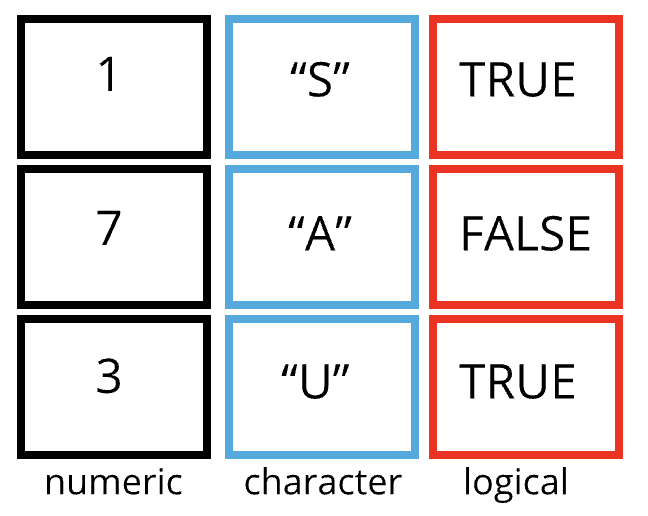
\includegraphics[width=0.8\linewidth]{img/data-frame} \caption{Structure of a data frame}\label{fig:data-frame}
\end{figure}

As we have seen above, data frames can be created by hand, but most commonly they are generated by the functions like \texttt{read.csv()}, \texttt{read\_csv()} or \texttt{read\_table()} and others. These functions essentiallly import the tables or spreadsheets from your hard drive (or the web). We will now demonstrate how to import tabular data using \texttt{read\_csv()}.

\hypertarget{importing-tabular-data}{%
\section{Importing tabular data}\label{importing-tabular-data}}

We will take a CSV file as example. \href{https://support.bigcommerce.com/articles/Public/What-is-a-CSV-file-and-how-do-I-save-my-spreadsheet-as-one}{What is a CSV file?}

You may know about \href{https://openpolicing.stanford.edu}{the Stanford Open Policing Project} and we will be working with a sample dataset from their repository (\url{https://openpolicing.stanford.edu/data/}). The sample I extracted contains information about traffic stops for black and white drivers in the state of Mississippi during January 2013 to mid-July of 2016.

First, we are going to use the R function \texttt{download.file()} to download the CSV file
that contains the traffic stop data, and we will use \texttt{read.csv()} to
load into memory the content of the CSV file as an object of class \texttt{data.frame}.

To download the data into your local \texttt{data/} subdirectory, run the following:

\begin{Shaded}
\begin{Highlighting}[]
\FunctionTok{download.file}\NormalTok{(}\StringTok{"http://bit.ly/MS\_trafficstops\_bw"}\NormalTok{, }\StringTok{"data/MS\_trafficstops\_bw.csv"}\NormalTok{)}
\end{Highlighting}
\end{Shaded}

You are going to load the data in R's memory using the function \texttt{read\_csv()} from the \texttt{readr} package, which is part of the \texttt{tidyverse}; learn more about the tidyverse collection of packages (here){[}\url{https://www.tidyverse.org/}{]}. \texttt{readr} gets installed as part as the \texttt{tidyverse} installation. When you load the \texttt{tidyverse} (\texttt{library(tidyverse)}), the core packages (the packages used in most data analyses) get loaded, including \texttt{readr.}

So lets make sure you have the \texttt{tidyverse} packages installed and loaded.

If you haven't done so already run the installation of \texttt{tidyverse} like this:

\begin{Shaded}
\begin{Highlighting}[]
\FunctionTok{install.packages}\NormalTok{(}\StringTok{"tidyverse"}\NormalTok{ , }\AttributeTok{dependencies =} \ConstantTok{TRUE}\NormalTok{) }\CommentTok{\# this is only necessary once}
\end{Highlighting}
\end{Shaded}

Then load \texttt{tidyverse} into memory like this:

\begin{Shaded}
\begin{Highlighting}[]
\FunctionTok{library}\NormalTok{(tidyverse) }\CommentTok{\# do this whenever you need to access functions from the tidyverse packages }
\end{Highlighting}
\end{Shaded}

You may have noticed that when you loaded the tidyverse package that you received the following message:

\texttt{──\ Conflicts\ ───────────────────────────────────────\ tidyverse\_conflicts()\ ──}
\texttt{✖\ dplyr::filter()\ masks\ stats::filter()}
\texttt{✖\ dplyr::lag()\ \ \ \ masks\ stats::lag()}
\texttt{ℹ\ Use\ the\ conflicted\ package\ to\ force\ all\ conflicts\ to\ become\ errors}

This presents a good opportunity to talk about conflicts. Certain packages we load can end up introducing function names that are already in use by pre-loaded R packages. For instance, when we load the \texttt{tidyverse} package below, we will introduce two conflicting functions: \texttt{filter()} and \texttt{lag()}. This happens because \texttt{filter} and \texttt{lag} are already functions used by the \texttt{stats} package (already pre-loaded in R). What will happen now is that if we, for example, call the \texttt{filter()} function, R will use the \texttt{dplyr::filter()} version and not the \texttt{stats::filter()} one. This happens because, if conflicted, \textbf{by default R uses the function from the most recently loaded package}. Conflicted functions may cause you some trouble in the future, so it is important that we are aware of them so that we can properly handle them, if we want.

To do so, we can use the following functions from the conflicted package:

\begin{itemize}
\tightlist
\item
  \texttt{conflicted::conflict\_scout()}: Shows us any conflicted functions.
\item
  \texttt{conflict\_prefer("function",\ "package\_prefered")}: Allows us to choose the default function we want from now on.
\end{itemize}

It is also important to know that we can, at any time, just call the function directly from the package we want, such as \texttt{stats::filter()}.

Ok. With that out of the way you are now ready to load the data.

\begin{Shaded}
\begin{Highlighting}[]
\NormalTok{stops }\OtherTok{\textless{}{-}} \FunctionTok{read\_csv}\NormalTok{(}\StringTok{"data/MS\_trafficstops\_bw.csv"}\NormalTok{)}
\end{Highlighting}
\end{Shaded}

\begin{verbatim}
#> Rows: 211211 Columns: 11
#> -- Column specification --------------------------------------------------------
#> Delimiter: ","
#> chr  (8): id, state, county_name, police_department, driver_gender, driver_r...
#> dbl  (1): county_fips
#> date (2): stop_date, driver_birthdate
#> 
#> i Use `spec()` to retrieve the full column specification for this data.
#> i Specify the column types or set `show_col_types = FALSE` to quiet this message.
\end{verbatim}

If you were to type in the code above, it is likely that the \texttt{read.csv()} (note the dot!) function would appear in the automatically populated list of functions. This function is different from the \texttt{read\_csv()} (note the underscore!) function, as it is included in the ``base'' packages that come pre-installed with R. Overall, \texttt{read.csv()} behaves similar to \texttt{read\_csv()}, with a few notable differences. First, \texttt{read.csv()} coerces column names with spaces and/or special characters to different names (e.g.~interview date becomes interview.date). Second, \texttt{read.csv()} stores data as a \textbf{data.frame}, where \texttt{read\_csv()} stores data as a \textbf{tibble}. We prefer tibbles because they have nice printing properties among other desirable qualities. Read more about tibbles \href{https://tibble.tidyverse.org/}{here.}

The second statement in the code above creates a data frame but doesn't output any data because, as you might recall, assignments (\texttt{\textless{}-}) don't display anything. (Note, however, that \texttt{read\_csv} may show informational text about the data frame that is created.)

So let's check out the data! We can type the name of the object \texttt{stops}:

\begin{Shaded}
\begin{Highlighting}[]
\NormalTok{stops}
\end{Highlighting}
\end{Shaded}

\begin{verbatim}
#> # A tibble: 211,211 x 11
#>    id            state stop_date  county_name      county_fips police_department
#>    <chr>         <chr> <date>     <chr>                  <dbl> <chr>            
#>  1 MS-2013-00001 MS    2013-01-01 Jones County           28067 Mississippi High~
#>  2 MS-2013-00002 MS    2013-01-01 Lauderdale Coun~       28075 Mississippi High~
#>  3 MS-2013-00003 MS    2013-01-01 Pike County            28113 Mississippi High~
#>  4 MS-2013-00004 MS    2013-01-01 Hancock County         28045 Mississippi High~
#>  5 MS-2013-00005 MS    2013-01-01 Holmes County          28051 Mississippi High~
#>  6 MS-2013-00006 MS    2013-01-01 Jackson County         28059 Mississippi High~
#>  7 MS-2013-00007 MS    2013-01-01 Jackson County         28059 Mississippi High~
#>  8 MS-2013-00008 MS    2013-01-01 Grenada County         28043 Mississippi High~
#>  9 MS-2013-00009 MS    2013-01-01 Holmes County          28051 Mississippi High~
#> 10 MS-2013-00010 MS    2013-01-01 Holmes County          28051 Mississippi High~
#> # i 211,201 more rows
#> # i 5 more variables: driver_gender <chr>, driver_birthdate <date>,
#> #   driver_race <chr>, violation_raw <chr>, officer_id <chr>
\end{verbatim}

\begin{Shaded}
\begin{Highlighting}[]
\DocumentationTok{\#\# Try also:}
\CommentTok{\# head(stops)}
\CommentTok{\# view(stops)}
\end{Highlighting}
\end{Shaded}

\texttt{read\_csv()} assumes that fields are delimited by commas. For other delimiters (like semicolon or tab) check out the help: \texttt{?read\_csv}

Note that \texttt{read\_csv()} loads the data as a so called ``tibble''. A tibble is an extended form of R data frames (as an object of multiple classes \texttt{tbl\_df}, \texttt{tbl}, and \texttt{data.frame}). This may sound confusing, but it is really not anything you typically with when working the data. In fact, it makes it a little more convenient.

As you may recall, a data frame in R is a special case of a list, and a representation of data where the columns are vectors that all have the same length. Because the columns are vectors, they all contain the same type of data (e.g., characters, integers, factors, etc.).

In this tibble you can see the type of data included in each column listed in an abbreviated fashion right below the column names. For instance, the \texttt{state} column is is of type character \texttt{\textless{}chr\textgreater{}}, the \texttt{stop\_date} is in \texttt{\textless{}date\textgreater{}} format and \texttt{county\_fips} are floating point numbers (abbreviated \texttt{\textless{}dbl\textgreater{}} for the word `double').

\hypertarget{inspecting-data-frames}{%
\section{Inspecting data frames}\label{inspecting-data-frames}}

When calling a \texttt{tbl\_df}object (like \texttt{stops} here), there is already a lot of information about our data frame being displayed such as the number of rows, the number of columns, the names of the columns, and as we just saw the class of data stored in each column. However, there are additional functions to extract this information from data frames. Here is a non-exhaustive list of some of these functions. Let's try them out!

We already saw how the functions \texttt{head()} and \texttt{str()} can be useful to check the
content and the structure of a data frame. Here is a non-exhaustive list of
functions to get a sense of the content/structure of the data. Let's try them out!

(Note: most of these functions are ``generic'', they can be used on other types of
objects besides data frames or tibbles.)

\begin{itemize}
\tightlist
\item
  Summary:

  \begin{itemize}
  \tightlist
  \item
    \texttt{str(stops)} - structure of the object and information about the class, length and
    content of each column
  \item
    \texttt{summary(stops)} - summary statistics for each column
  \item
    \texttt{glimpse(stops)} - returns the number of columns and rows of the tibble, the names and class of each column, and previews as many values will fit on the screen. Unlike the other inspecting functions listed above, \texttt{glimpse()} is not a `base R' function so you need to have the \texttt{dplyr} or \texttt{tibble} packages loaded to be able to execute it.
  \end{itemize}
\item
  Size:

  \begin{itemize}
  \tightlist
  \item
    \texttt{dim(stops)} - returns a vector with the number of rows in the first element,
    and the number of columns as the second element (the \textbf{dim}ensions of
    the object)
  \item
    \texttt{nrow(stops)} - returns the number of rows
  \item
    \texttt{ncol(stops)} - returns the number of columns
  \item
    \texttt{length(stops)} - returns number of columns
  \end{itemize}
\item
  Content:

  \begin{itemize}
  \tightlist
  \item
    \texttt{head(stops)} - shows the first 6 rows
  \item
    \texttt{tail(stops)} - shows the last 6 rows
  \end{itemize}
\item
  Names:

  \begin{itemize}
  \tightlist
  \item
    \texttt{names(stops)} - returns the column names (synonym of \texttt{colnames()} for \texttt{data.frame}
    objects)
  \item
    \texttt{rownames(stops)} - returns the row names
  \end{itemize}
\end{itemize}

\begin{quote}
Challenge

Based on the output of \texttt{str(stops)}, can you answer the following questions?

\begin{itemize}
\tightlist
\item
  What is the class of the object \texttt{stops}?
\item
  How many rows and how many columns are in this object?
\item
  How many counties have been recorded in this dataset?
\end{itemize}
\end{quote}

\hypertarget{indexing-and-subsetting-data-frames}{%
\section{Indexing and subsetting data frames}\label{indexing-and-subsetting-data-frames}}

Our stops data frame has rows and columns (it has 2 dimensions), if we want to
extract some specific data from it, we need to specify the ``coordinates'' (i.e., indices) we want from it. Row numbers come first, followed by column numbers.

\begin{Shaded}
\begin{Highlighting}[]
\DocumentationTok{\#\# first element in the first column of the tibble}
\NormalTok{stops[}\DecValTok{1}\NormalTok{, }\DecValTok{1}\NormalTok{]}
\DocumentationTok{\#\# first element in the 6th column of the tibble }
\NormalTok{stops[}\DecValTok{1}\NormalTok{, }\DecValTok{6}\NormalTok{]}
\DocumentationTok{\#\# first column of the tibble}
\NormalTok{stops[}\DecValTok{1}\NormalTok{]}
\DocumentationTok{\#\# first column of the tibble (as a vector)}
\NormalTok{stops[[}\DecValTok{1}\NormalTok{]]}

\DocumentationTok{\#\# the 3rd row of the tibble}
\NormalTok{stops[}\DecValTok{3}\NormalTok{, ]}
\DocumentationTok{\#\# first three elements in the 7th column of the tibble}
\NormalTok{stops[}\DecValTok{1}\SpecialCharTok{:}\DecValTok{3}\NormalTok{, }\DecValTok{7}\NormalTok{]}
\DocumentationTok{\#\# equivalent to head(stops) }
\NormalTok{stops[}\DecValTok{1}\SpecialCharTok{:}\DecValTok{6}\NormalTok{, ]}

\DocumentationTok{\#\# Excludig with \textquotesingle{}{-}\textquotesingle{}}
\DocumentationTok{\#\# The whole tibble, except the first column}
\NormalTok{stops[, }\SpecialCharTok{{-}}\DecValTok{1}\NormalTok{]          }
\DocumentationTok{\#\# equivalent to head(stops)  }
\NormalTok{stops[}\SpecialCharTok{{-}}\FunctionTok{c}\NormalTok{(}\DecValTok{7}\SpecialCharTok{:}\FunctionTok{nrow}\NormalTok{(stops)),]}
\end{Highlighting}
\end{Shaded}

Subsetting a \texttt{tibble} with \texttt{{[}} always results in a tibble. However, note that different ways of specifying these coordinates lead to results with different classes. Below are some example for \texttt{data.frame} objects.

\begin{Shaded}
\begin{Highlighting}[]
\NormalTok{stops\_df }\OtherTok{\textless{}{-}} \FunctionTok{as.data.frame}\NormalTok{(stops)}
\NormalTok{stops\_df[}\DecValTok{1}\NormalTok{, }\DecValTok{1}\NormalTok{]   }\CommentTok{\# first element in the first column of the data frame (as a vector)}
\NormalTok{stops\_df[, }\DecValTok{1}\NormalTok{]    }\CommentTok{\# first column in the data frame (as a vector)}
\NormalTok{stops\_df[}\DecValTok{1}\NormalTok{]      }\CommentTok{\# first column in the data frame (as a data.frame)}
\end{Highlighting}
\end{Shaded}

An alternative to subsetting \texttt{tibbles} (and data frames) is to calling their column names directly.

\begin{Shaded}
\begin{Highlighting}[]
\NormalTok{stops[}\StringTok{"violation\_raw"}\NormalTok{]       }\CommentTok{\# Result is a tibble}
\NormalTok{stops[, }\StringTok{"violation\_raw"}\NormalTok{]     }\CommentTok{\# Result is a tibble}
\NormalTok{stops[[}\StringTok{"violation\_raw"}\NormalTok{]]     }\CommentTok{\# Result is a vector}
\NormalTok{stops}\SpecialCharTok{$}\NormalTok{violation\_raw          }\CommentTok{\# Result is a vector}
\end{Highlighting}
\end{Shaded}

RStudio knows about the columns in your data frame, so you can take advantage of the autocompletion feature to get the full and correct column name.

\begin{quote}
Challenge

\begin{enumerate}
\def\labelenumi{\arabic{enumi}.}
\item
  Create a \texttt{tibble} (\texttt{stops\_200}) containing only the observations from
  row 200 of the \texttt{stops} dataset.
\item
  Notice how \texttt{nrow()} gave you the number of rows in a \texttt{tibble}?

  \begin{itemize}
  \tightlist
  \item
    Use that number to pull out just that last row in the data frame.
  \item
    Compare that with what you see as the last row using \texttt{tail()} to make
    sure it's meeting expectations.
  \item
    Pull out that last row using \texttt{nrow()} instead of the row number.
  \item
    Create a new data frame object (\texttt{stops\_last}) from that last row.
  \end{itemize}
\item
  Use \texttt{nrow()} to extract the row that is in the middle of the data
  frame. Store the content of this row in an object named \texttt{stops\_middle}.
\item
  Combine \texttt{nrow()} with the \texttt{-} notation above to reproduce the behavior of
  \texttt{head(stops)} keeping just the first through 6th rows of the stops
  dataset.
\end{enumerate}
\end{quote}

\hypertarget{conditional-subsetting-1}{%
\section{Conditional subsetting}\label{conditional-subsetting-1}}

A very common need when working with tables is the need to extract a subset of a data frame based on certain conditions, depending on the actualcontent of the table. For example, we may want to look only at traffic stops in Webster County. In this case we can use logical conditions, exactly like we did above with vector subsetting. In base R this can be done like this:

\begin{Shaded}
\begin{Highlighting}[]
\CommentTok{\# the condition:}
\CommentTok{\# returns a logical vector of the length of the column}
\NormalTok{stops}\SpecialCharTok{$}\NormalTok{county\_name }\SpecialCharTok{==} \StringTok{"Webster County"} 

\CommentTok{\# use this vector to extract rows and all columns}
\CommentTok{\# note the comma: we want *all* columns}
\NormalTok{stops[stops}\SpecialCharTok{$}\NormalTok{county\_name }\SpecialCharTok{==} \StringTok{"Webster County"}\NormalTok{, ] }

\CommentTok{\# assign extract to a new data frame}
\NormalTok{Webster\_stops }\OtherTok{\textless{}{-}}\NormalTok{ stops[stops}\SpecialCharTok{$}\NormalTok{county\_name }\SpecialCharTok{==} \StringTok{"Webster County"}\NormalTok{, ]}
\end{Highlighting}
\end{Shaded}

This is also a possibility (but slower):

\begin{Shaded}
\begin{Highlighting}[]
\NormalTok{Webster\_stops }\OtherTok{\textless{}{-}} \FunctionTok{subset}\NormalTok{(stops, county\_name }\SpecialCharTok{==} \StringTok{"Webster County"}\NormalTok{)}
\FunctionTok{nrow}\NormalTok{(Webster\_stops) }\CommentTok{\# 393 stops in Webster County!}
\end{Highlighting}
\end{Shaded}

\begin{verbatim}
#> [1] 156
\end{verbatim}

\begin{Shaded}
\begin{Highlighting}[]
\CommentTok{\# and if we wanted to see the breakdown by race:}
\FunctionTok{table}\NormalTok{(Webster\_stops}\SpecialCharTok{$}\NormalTok{driver\_race)}
\end{Highlighting}
\end{Shaded}

\begin{verbatim}
#> 
#> Black White 
#>    59    97
\end{verbatim}

These commands are from the R base package. In the R Data Wrangling workshop we will discuss a different way of subsetting using functions from the \texttt{tidyverse} package.

\begin{quote}
Challenge

\begin{itemize}
\tightlist
\item
  Use subsetting to extract stops in Hancock, Harrison, and Jackson Counties into a separate data frame \texttt{coastal\_counties}.
\item
  Using \texttt{coastal\_counties}, count the total number of Black and White drivers in the coastal counties.
\item
  Bonus: Count the total number of Black and White drivers in the entire \texttt{stops} dataset. How does the ratio of Black to White stops in the three coastal counties compare to the same ratio for stops in the entire state of Mississippi?
\end{itemize}
\end{quote}

\hypertarget{adding-and-removing-rows-and-columns}{%
\section{Adding and removing rows and columns}\label{adding-and-removing-rows-and-columns}}

To add a new column to the data frame we can use the \texttt{cbind()} function There also is a \texttt{bind\_cols()} function from \texttt{dplyr} package (part of the \texttt{tidyverse}). An important difference with \texttt{bind\_cols()} is that it displays an error message when you try to combine with vector that has fewer or more elements than the number of rows in the table. \texttt{cbind()} on the other hand, silently repeats values or rows, so you might introduce errors and be unaware of it.

\begin{Shaded}
\begin{Highlighting}[]
\NormalTok{id\_column }\OtherTok{\textless{}{-}} \DecValTok{1}\SpecialCharTok{:}\FunctionTok{nrow}\NormalTok{(stops) }\CommentTok{\# create a unique ID number for each row}
\NormalTok{stops\_with\_id }\OtherTok{\textless{}{-}} \FunctionTok{cbind}\NormalTok{(stops, id\_column) }
\FunctionTok{glimpse}\NormalTok{(stops\_with\_id)}
\end{Highlighting}
\end{Shaded}

\begin{verbatim}
#> Rows: 211,211
#> Columns: 12
#> $ id                <chr> "MS-2013-00001", "MS-2013-00002", "MS-2013-00003", "~
#> $ state             <chr> "MS", "MS", "MS", "MS", "MS", "MS", "MS", "MS", "MS"~
#> $ stop_date         <date> 2013-01-01, 2013-01-01, 2013-01-01, 2013-01-01, 201~
#> $ county_name       <chr> "Jones County", "Lauderdale County", "Pike County", ~
#> $ county_fips       <dbl> 28067, 28075, 28113, 28045, 28051, 28059, 28059, 280~
#> $ police_department <chr> "Mississippi Highway Patrol", "Mississippi Highway P~
#> $ driver_gender     <chr> "M", "M", "M", "M", "M", "F", "F", "F", "M", "M", "M~
#> $ driver_birthdate  <date> 1950-06-14, 1967-04-06, 1974-04-15, 1981-03-23, 199~
#> $ driver_race       <chr> "Black", "Black", "Black", "White", "White", "White"~
#> $ violation_raw     <chr> "Seat belt not used properly as required", "Careless~
#> $ officer_id        <chr> "J042", "B026", "M009", "K035", "D028", "K023", "K03~
#> $ id_column         <int> 1, 2, 3, 4, 5, 6, 7, 8, 9, 10, 11, 12, 13, 14, 15, 1~
\end{verbatim}

Alternatively, we can also add a new column adding the new column name after the \texttt{\$} sign then assigning the value, like below. \textbf{Note that this will change the original data frame, which you may not always want to do.}

\begin{Shaded}
\begin{Highlighting}[]
\NormalTok{stops}\SpecialCharTok{$}\NormalTok{row\_numbers }\OtherTok{\textless{}{-}} \FunctionTok{c}\NormalTok{(}\DecValTok{1}\SpecialCharTok{:}\FunctionTok{nrow}\NormalTok{(stops))}
\NormalTok{stops}\SpecialCharTok{$}\NormalTok{all\_false }\OtherTok{\textless{}{-}} \ConstantTok{FALSE}  \CommentTok{\# what do you think will happen here?}
\end{Highlighting}
\end{Shaded}

There is an equivalent function, \texttt{rbind()} to add a new row to a data frame. I use this far less frequently than the column equivalent. The one thing to keep in mind is that the row to be added to the data frame needs to match the order and type of columns in the data frame. Remember that R's way to store multiple different data types in one object is a \texttt{list}. So if we wanted to add a new row to \texttt{stops} we would say:

\begin{Shaded}
\begin{Highlighting}[]
\NormalTok{new\_row }\OtherTok{\textless{}{-}} \FunctionTok{data.frame}\NormalTok{(}\AttributeTok{id=}\StringTok{"MS{-}2017{-}12345"}\NormalTok{, }\AttributeTok{state=}\StringTok{"MS"}\NormalTok{, }\AttributeTok{stop\_date=}\StringTok{"2017{-}08{-}24"}\NormalTok{,}
                \AttributeTok{county\_name=}\StringTok{"Tallahatchie County"}\NormalTok{, }\AttributeTok{county\_fips=}\DecValTok{12345}\NormalTok{,}
                \AttributeTok{police\_department=}\StringTok{"MSHP"}\NormalTok{, }\AttributeTok{driver\_gender=}\StringTok{"F"}\NormalTok{, }\AttributeTok{driver\_birthdate=}\StringTok{"1999{-}06{-}14"}\NormalTok{,}
                \AttributeTok{driver\_race=}\StringTok{"Hispanic"}\NormalTok{, }\AttributeTok{violation\_raw=}\StringTok{"Speeding"}\NormalTok{, }\AttributeTok{officer\_id=}\StringTok{"ABCD"}\NormalTok{)}

\NormalTok{stops\_withnewrow }\OtherTok{\textless{}{-}} \FunctionTok{rbind}\NormalTok{(stops, new\_row)}
\FunctionTok{tail}\NormalTok{(stops\_withnewrow)}
\end{Highlighting}
\end{Shaded}

\begin{verbatim}
#> # A tibble: 6 x 11
#>   id    state stop_date  county_name county_fips police_department driver_gender
#>   <chr> <chr> <date>     <chr>             <dbl> <chr>             <chr>        
#> 1 MS-2~ MS    2016-07-09 George Cou~       28039 Mississippi High~ M            
#> 2 MS-2~ MS    2016-07-10 Copiah Cou~       28029 Mississippi High~ M            
#> 3 MS-2~ MS    2016-07-11 Grenada Co~       28043 Mississippi High~ M            
#> 4 MS-2~ MS    2016-07-14 Copiah Cou~       28029 Mississippi High~ F            
#> 5 MS-2~ MS    2016-07-14 Copiah Cou~       28029 Mississippi High~ M            
#> 6 MS-2~ MS    2017-08-24 Tallahatch~       12345 MSHP              F            
#> # i 4 more variables: driver_birthdate <date>, driver_race <chr>,
#> #   violation_raw <chr>, officer_id <chr>
\end{verbatim}

Equivalently there is a \texttt{bind\_rows} function available in \texttt{tidyverse}. One of the main reasons for using \texttt{bind\_rows} over \texttt{rbind} is to combine two data frames having different number of columns. \texttt{rbind} throws an error in such a case whereas \texttt{bind\_rows} assigns ``NA'' to those rows of columns missing in one of the data frames where the value is not provided by the data frames. \href{https://stackoverflow.com/a/59482527}{Here is a systematic review of differences between the two.}

There is also \texttt{add\_row} fro the \texttt{tibble} package which allows you to specify where to insert the row. You can find out more with \texttt{?add\_row}.

A convenient function to know about is \texttt{na.omit()}. It will remove all rows from a data frame that have at least one column with \texttt{NA} values. The function \texttt{drop\_na()} from \texttt{tidyverse} works similarly and lets you name specific columns with NA.

\begin{quote}
Challenge

\begin{itemize}
\tightlist
\item
  Given the following data frame:
\end{itemize}

\begin{Shaded}
\begin{Highlighting}[]
\NormalTok{dfr }\OtherTok{\textless{}{-}} \FunctionTok{data.frame}\NormalTok{(}\AttributeTok{col\_1 =} \FunctionTok{c}\NormalTok{(}\DecValTok{1}\SpecialCharTok{:}\DecValTok{3}\NormalTok{), }
                  \AttributeTok{col\_2 =} \FunctionTok{c}\NormalTok{(}\ConstantTok{NA}\NormalTok{, }\ConstantTok{NA}\NormalTok{, }\StringTok{"b"}\NormalTok{), }
                  \AttributeTok{col\_3 =} \FunctionTok{c}\NormalTok{(}\ConstantTok{TRUE}\NormalTok{, }\ConstantTok{NA}\NormalTok{, }\ConstantTok{FALSE}\NormalTok{))}
\end{Highlighting}
\end{Shaded}

What would you expect the following commands to return?

\begin{Shaded}
\begin{Highlighting}[]
\FunctionTok{nrow}\NormalTok{(dfr)}
\FunctionTok{nrow}\NormalTok{(}\FunctionTok{na.omit}\NormalTok{(dfr))}
\end{Highlighting}
\end{Shaded}
\end{quote}

\hypertarget{categorical-data-factors}{%
\section{Categorical data: Factors}\label{categorical-data-factors}}

Factors are very useful and are actually
something that make R particularly well suited to working with data, so we're
going to spend a little time introducing them.

Factors are used to represent categorical data. Factors can be ordered or
unordered, and understanding them is necessary for statistical analysis and for
plotting.

Factors are stored as integers, and have labels (text) associated with these
unique integers. While factors look (and often behave) like character vectors,
they are actually integers under the hood, and you need to be careful when
treating them like strings.

Once created, factors can only contain a pre-defined set of values, known as
\emph{levels}. By default, R always sorts \emph{levels} in alphabetical order. For
instance, if you have a factor with 3 levels:

\begin{Shaded}
\begin{Highlighting}[]
\NormalTok{priority }\OtherTok{\textless{}{-}} \FunctionTok{factor}\NormalTok{(}\FunctionTok{c}\NormalTok{(}\StringTok{"low"}\NormalTok{, }\StringTok{"high"}\NormalTok{, }\StringTok{"medium"}\NormalTok{, }\StringTok{"low"}\NormalTok{, }\StringTok{"high"}\NormalTok{))}
\end{Highlighting}
\end{Shaded}

R will assign \texttt{1} to the level \texttt{"high"} and \texttt{2} to the level \texttt{"low"} and \texttt{3} to the level \texttt{low} (because it orders alphabetically, not according to position in the vector). You can check this by using the function \texttt{levels()}, and check the number of levels using \texttt{nlevels()}:

\begin{Shaded}
\begin{Highlighting}[]
\FunctionTok{levels}\NormalTok{(priority)}
\FunctionTok{nlevels}\NormalTok{(priority)}
\end{Highlighting}
\end{Shaded}

Sometimes, the order of the factors does not matter, other times you might want
to specify the order because it is meaningful (e.g., ``low'', ``medium'', ``high''),
it improves your visualization, or it is required by a particular type of
analysis. Here, one way to reorder our levels in the \texttt{priority} vector would be:

\begin{Shaded}
\begin{Highlighting}[]
\NormalTok{priority }\CommentTok{\# current order}
\end{Highlighting}
\end{Shaded}

\begin{verbatim}
#> [1] low    high   medium low    high  
#> Levels: high low medium
\end{verbatim}

\begin{Shaded}
\begin{Highlighting}[]
\NormalTok{priority }\OtherTok{\textless{}{-}} \FunctionTok{factor}\NormalTok{(priority, }\AttributeTok{levels =} \FunctionTok{c}\NormalTok{(}\StringTok{"high"}\NormalTok{, }\StringTok{"medium"}\NormalTok{, }\StringTok{"low"}\NormalTok{))}
\NormalTok{priority }\CommentTok{\# after re{-}ordering}
\end{Highlighting}
\end{Shaded}

\begin{verbatim}
#> [1] low    high   medium low    high  
#> Levels: high medium low
\end{verbatim}

In R's memory, these factors are represented by integers (1, 2, 3), but are more
informative than integers because factors are self describing: \texttt{"high"},
\texttt{"medium"} and \texttt{"low"} is more descriptive than \texttt{1}, \texttt{2}, \texttt{3}. Which one is ``low''? You wouldn't
be able to tell just from the integer data. Factors, on the other hand, have
this information built in.

\hypertarget{converting-factors}{%
\subsection{Converting factors}\label{converting-factors}}

If you need to convert a factor to a character vector, you use
\texttt{as.character(x)}.

\begin{Shaded}
\begin{Highlighting}[]
\FunctionTok{as.character}\NormalTok{(priority)}
\end{Highlighting}
\end{Shaded}

It is a little is a little trickier to convert factors where the levels appear as numbers, such or years, for example, to numbers.One method is to
convert factors to characters and then numbers. Another method is to use the \texttt{levels()} function. Compare:

\begin{Shaded}
\begin{Highlighting}[]
\NormalTok{y }\OtherTok{\textless{}{-}} \FunctionTok{factor}\NormalTok{(}\FunctionTok{c}\NormalTok{(}\DecValTok{1990}\NormalTok{, }\DecValTok{1983}\NormalTok{, }\DecValTok{1977}\NormalTok{, }\DecValTok{1998}\NormalTok{, }\DecValTok{1990}\NormalTok{))}
\FunctionTok{as.numeric}\NormalTok{(y)               }\CommentTok{\# wrong! and there is no warning...}
\FunctionTok{as.numeric}\NormalTok{(}\FunctionTok{as.character}\NormalTok{(y)) }\CommentTok{\# works...}
\FunctionTok{as.numeric}\NormalTok{(}\FunctionTok{levels}\NormalTok{(y))[y]    }\CommentTok{\# The recommended way.}
\end{Highlighting}
\end{Shaded}

Notice that in the \texttt{levels()} approach, three important steps occur:

\begin{itemize}
\tightlist
\item
  We obtain all the factor levels using \texttt{levels(y)}
\item
  We convert these levels to numeric values using \texttt{as.numeric(levels(y))}
\item
  We then access these numeric values using the underlying integers of the vector \texttt{y} as indices inside the square brackets
\end{itemize}

\hypertarget{renaming-factors}{%
\subsection{Renaming factors}\label{renaming-factors}}

When your data is stored as a factor, you can use the \texttt{plot()} function to get a quick glance at the number of observations represented by each factor
level. Let's look at the number of black and white drivers in the \texttt{stops} dataset:

\begin{Shaded}
\begin{Highlighting}[]
\CommentTok{\# We create a new variable with the column "driver\_race" as a factor}
\NormalTok{race }\OtherTok{\textless{}{-}}\NormalTok{ stops}\SpecialCharTok{$}\NormalTok{driver\_race}
\NormalTok{race }\OtherTok{\textless{}{-}} \FunctionTok{factor}\NormalTok{(race)}
\FunctionTok{plot}\NormalTok{(race)}
\end{Highlighting}
\end{Shaded}

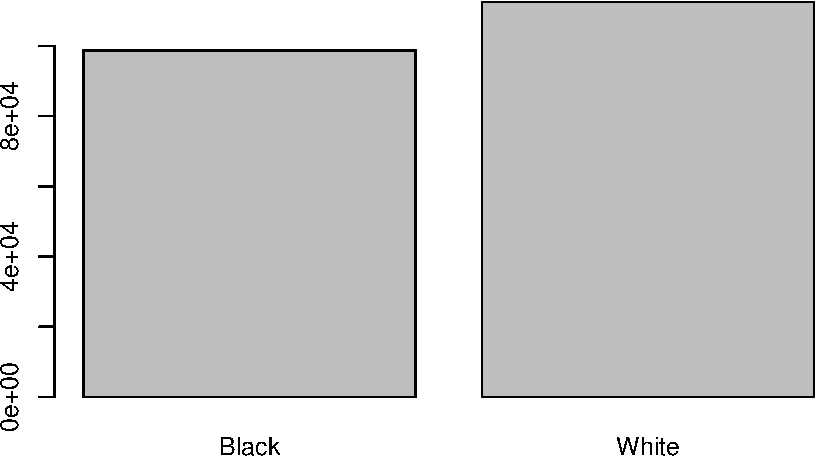
\includegraphics{R-intro_files/figure-latex/driver-race-barplot-1.pdf}

This looks good, however, \texttt{plot} silently ignores NAs and we would like to know if there are any:

\begin{Shaded}
\begin{Highlighting}[]
\CommentTok{\# We create a new variable with the column "driver\_race" as a factor}
\FunctionTok{sum}\NormalTok{(}\FunctionTok{is.na}\NormalTok{(race))}
\end{Highlighting}
\end{Shaded}

There seem to be a number of individuals for which the race information hasn't been recorded. Additionally, for these individuals, there is no label to indicate that the information is missing. Let's rename this label to something more meaningful:

\begin{Shaded}
\begin{Highlighting}[]
\DocumentationTok{\#\# Let\textquotesingle{}s recreate the vector from the data frame column "memb\_assoc"}
\NormalTok{race }\OtherTok{\textless{}{-}}\NormalTok{ stops}\SpecialCharTok{$}\NormalTok{driver\_race}

\DocumentationTok{\#\# replace the missing data with "unknown"}
\NormalTok{race[}\FunctionTok{is.na}\NormalTok{(race)] }\OtherTok{\textless{}{-}} \StringTok{\textquotesingle{}Missing\textquotesingle{}}

\DocumentationTok{\#\# convert it into a factor}
\NormalTok{race }\OtherTok{\textless{}{-}} \FunctionTok{as.factor}\NormalTok{(race)}

\DocumentationTok{\#\# let\textquotesingle{}s see what it looks like}
\FunctionTok{plot}\NormalTok{(race)}
\end{Highlighting}
\end{Shaded}

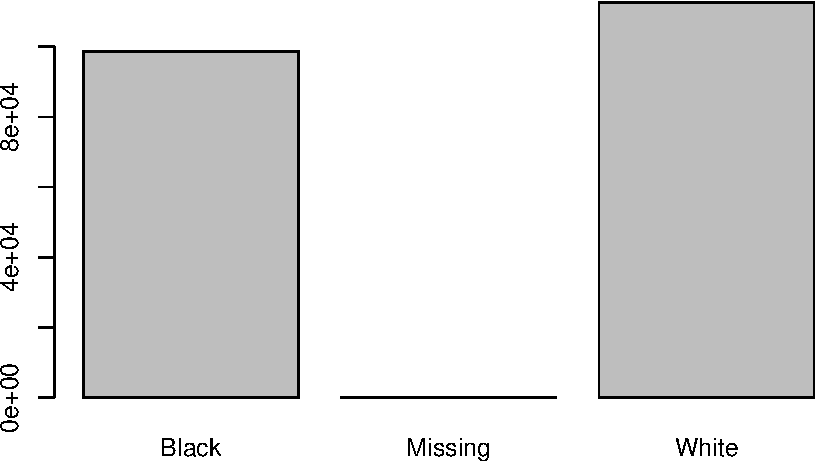
\includegraphics{R-intro_files/figure-latex/unnamed-chunk-94-1.pdf}

\begin{quote}
Challenge

\begin{itemize}
\tightlist
\item
  Rename ``Black'' to ``African American''.
\item
  Now that we have renamed the factor level to ``Missing'', can you recreate the
  barplot such that ``Missing'' is last (to the right)?
\end{itemize}
\end{quote}

---\textgreater{}

\hypertarget{date-formats}{%
\section{Date Formats}\label{date-formats}}

One of the most common issues that new (and experienced!) R users have is converting
date and time information into a variable that is appropriate and usable during
analyses. If you have control over your data it might be useful to ensure that each component of your date is stored as a separate
variable, i.e a separate column for day, month, and year. However, often we do not have control and the date is stored in one single column and with varying order and separating characters between its components.

Using \texttt{str()}, we can see that both dates in our data frame \texttt{stop\_date} and \texttt{driver\_birthdate} are each stored in one column.

\begin{Shaded}
\begin{Highlighting}[]
\FunctionTok{str}\NormalTok{(stops)}
\end{Highlighting}
\end{Shaded}

As an example for how to work with dates let us see if there are seasonal differences in the number of traffic stops.

We're going to be using the \texttt{ymd()} function from the package \textbf{\texttt{lubridate}}. This
function is designed to take a vector representing year, month, and day and convert
that information to a POSIXct vector. POSIXct is a class of data recognized by R as
being a date or date and time. The argument that the function requires is relatively
flexible, but, as a best practice, is a character vector formatted as ``YYYY-MM-DD''.

Start by loading the required package:

\begin{Shaded}
\begin{Highlighting}[]
\FunctionTok{library}\NormalTok{(lubridate)}
\end{Highlighting}
\end{Shaded}

\texttt{read\_csv()} has already recognized the Date format of the column when we read the table in earlier.

\begin{Shaded}
\begin{Highlighting}[]
\NormalTok{stop\_date }\OtherTok{\textless{}{-}}\NormalTok{ stops}\SpecialCharTok{$}\NormalTok{stop\_date}
\FunctionTok{str}\NormalTok{(stop\_date) }\CommentTok{\# notice the \textquotesingle{}Date\textquotesingle{} class}
\end{Highlighting}
\end{Shaded}

We can now take advantage of different functions to extract year, month, and day: \texttt{year()}, \texttt{month()}, and \texttt{day()} like so:

\begin{Shaded}
\begin{Highlighting}[]
\NormalTok{stop\_year }\OtherTok{\textless{}{-}} \FunctionTok{year}\NormalTok{(stop\_date) }\CommentTok{\# extract the year}

\CommentTok{\# convert year to factor to plot}
\FunctionTok{plot}\NormalTok{(}\FunctionTok{factor}\NormalTok{(stop\_year)) }
\end{Highlighting}
\end{Shaded}

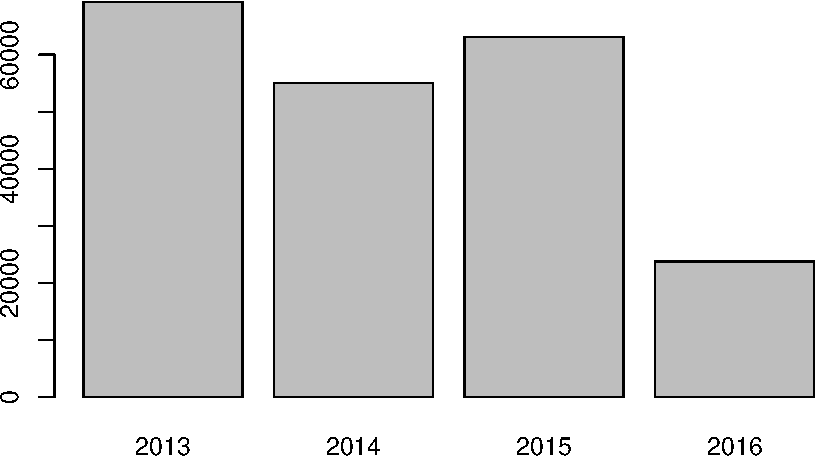
\includegraphics{R-intro_files/figure-latex/yearly-stops-1.pdf}

\begin{quote}
Challenge

\begin{itemize}
\tightlist
\item
  Are there more stops in certain months of the year or certain days of the month?
\end{itemize}
\end{quote}

\begin{Shaded}
\begin{Highlighting}[]
\FunctionTok{plot}\NormalTok{(}\FunctionTok{factor}\NormalTok{(}\FunctionTok{day}\NormalTok{(stop\_date)))}
\end{Highlighting}
\end{Shaded}

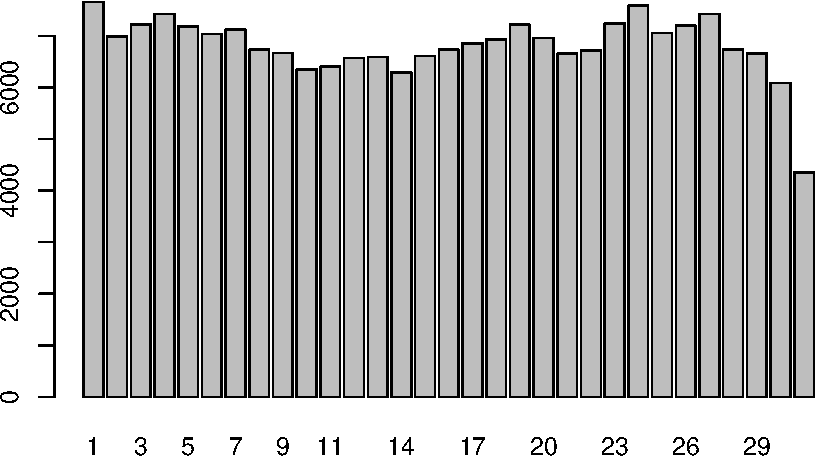
\includegraphics{R-intro_files/figure-latex/plot-seasonal-stops-2.pdf}
---\textgreater{}

\begin{quote}
Challenge

\begin{itemize}
\tightlist
\item
  Determine the age of the driver in years (approximate) at the time of the stop:
\item
  Extract \texttt{driver\_birthdate} into a vector \texttt{birth\_date}
\item
  Create a new vector \texttt{age} with the driver's age at the time of the stop in years
\item
  Coerce \texttt{age} to a factor and use the \texttt{plot} function to check your results. What do you find?
\end{itemize}
\end{quote}

\begin{Shaded}
\begin{Highlighting}[]
\CommentTok{\# or}
\FunctionTok{hist}\NormalTok{(age)}
\end{Highlighting}
\end{Shaded}

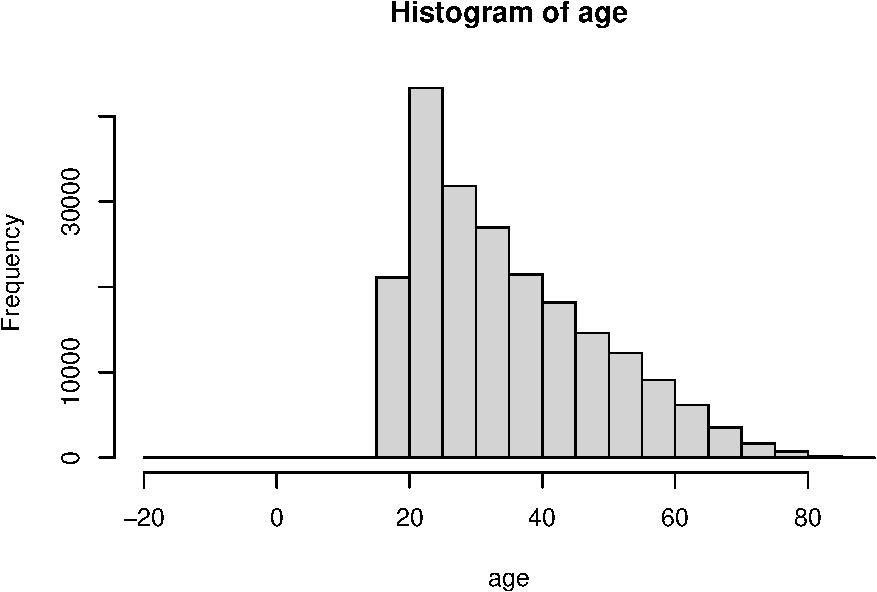
\includegraphics{R-intro_files/figure-latex/calculate-age-answer-2.pdf}
---\textgreater{}

  \bibliography{book.bib,packages.bib}

\end{document}
